\documentclass{article}
\usepackage{amsmath}
\usepackage{amssymb}
\usepackage{graphicx}
\usepackage{float}
\usepackage[margin=1in]{geometry}
\usepackage{setspace}
\onehalfspacing
\usepackage{makeidx}
\usepackage[hidelinks]{hyperref}
\usepackage{indentfirst}
\usepackage{caption}
\usepackage{fancyhdr}
\usepackage[T1]{fontenc}
\usepackage[backend=bibtex]{biblatex}
\usepackage[spanish]{babel}
\usepackage{svg}

\newlength{\drop}

% Sangría
\setlength{\parindent}{1.2cm}

%Títulos de los índices
\renewcommand{\listfigurename}{Índice de Figuras}
\renewcommand{\contentsname}{Índice}
\renewcommand{\listtablename}{Índice de Tablas}

\begin{document}
%Carátula
\begin{titlepage}
    %\drop=0.05\textheight
    \vspace{-0.5cm}
    % Encabezado
    \noindent
    \begin{tabular}{@{}p{0.5\textwidth}@{\hspace{0.05\textwidth}}p{0.45\textwidth}@{}}
    \begin{flushleft}
    Universidad Nacional de Córdoba \\
    Facultad de Ciencias Exactas, Físicas y Naturales \\
    Escuela de Ingeniería Electrónica
    \end{flushleft} &
    \begin{flushright}
    \hspace{-0.5cm}
\includegraphics[width=5.7cm]{logo.png} 
    \end{flushright}
    \end{tabular}
    \newline
    \rule{\textwidth}{0.4pt} % Línea debajo del encabezado
        
    
    %\vspace{1cm} % Espacio adicional
    
    \centering
    \vspace*{5cm} % Centra verticalmente el título
    \rule{\textwidth}{1.6pt}\vspace*{-\baselineskip}\vspace*{2pt}
    \rule{\textwidth}{0.4pt}\\
    {\LARGE \textbf{Trabajo Práctico N°1}\\
    Circuito Sintonizado Simple \\[0.3\baselineskip]}
    \rule{\textwidth}{0.4pt}\vspace*{-\baselineskip}\vspace{3.2pt}
    \rule{\textwidth}{1.6pt}\\
    \vspace*{\fill} % Espacio adicional después del título

    % Información del autor
    \begin{minipage}[b]{0.4\textwidth}
    \begin{flushleft}
    \textbf{Alumno:}\\
    Villar, Federico Ignacio \\
    DNI: 42.720.483
    \end{flushleft}
    \end{minipage}
    \begin{minipage}[b]{0.5\textwidth}
    \begin{flushright}
    \textbf{Docentes:}\\
    Ing. Amado, José \\
    Ing. Bruni, Rodrigo \\
    Ing. Dadam, Federico
    \end{flushright}
    \end{minipage}

    
\end{titlepage}


%Encabezado y pie de página
\pagestyle{fancy}
\fancyhf{}
\fancyhead[L]{\leftmark} % Sección actual en la izquierda
\fancyhead[R]{EAIII - FCEFyN UNC} % Texto en la derecha
\renewcommand{\headrulewidth}{0.4pt} % Grosor de la línea inferior del encabezado
\fancyfoot[L]{\textbf{Villar, Federico Ignacio}} % Nombre en la izquierda del pie de página
\fancyfoot[R]{\thepage} % Número de página en la derecha del pie de página
\renewcommand{\footrulewidth}{0.4pt} % Grosor de la línea superior del pie 

%Indices
\thispagestyle{empty}
\tableofcontents
\newpage
\thispagestyle{empty}
\listoffigures
\newpage
\thispagestyle{empty}
\listoftables

%Introducción
\newpage
\thispagestyle{empty}
\section{Introducción}
En el siguiente informe se detallará el desarrollo de un acoplamiento sintonizado simple para una determinada frecuencia en $MHz$. Se diseñó un circuito en función de especificaciones dadas en clase, siendo éstas las siguientes:
\begin{itemize}
    \item $f_o=13 MHz$
	\item $Z_g=50 \Omega$
	\item $Z_L=1 k\Omega$
	\item $Q_c=10$
\end{itemize}
\noindent Se pretende mostrar las diferentes etapas del diseño, materiales, métodos, así como también un análisis de resultados y un marco teórico a fin de ilustrar el tema en general.

%Marco Teórico
\newpage
\section{Marco Teórico}
\subsection{Acoplamiento sintonizado simple}
Se parte del diseño de un circuito resonador RLC en paralelo, cuyos componentes resistivo, inductivo y capacitivo son definidos de forma genérica con la inicial de la magnitud que representan. Es importante también mencionar que la fuente de tensión del sistema es modelada de forma no ideal, es decir, que posee una resistencia interna, llamada Rg. El esquema al que se hace referencia puede verse a continuación.
%% ------- Figura 1 ------- %%
\begin{figure}[H]
\centering
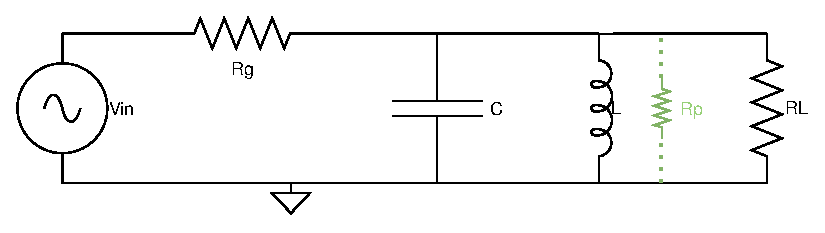
\includegraphics[width=0.7\textwidth]{./img/figura1.eps}
\caption{Circuito resonador RLC en paralelo.}
\label{fig:circuito}
\end{figure}
\noindent Cuando se trabaja con inductores y capacitores, existe la llamada condición de resonancia, que se da en la frecuencia para la cual, las reactancias capacitivas e inductivas del circuito son iguales, lo que hace que al calcular la reactancia compleja total se anule el término complejo de la expresión de la impedancia. Esto parte del supuesto de que la resistencia como tal es puramente real, algo que en la vida real no es del todo cierto, suelen tener cierto componente inductivo.
Obviando ahora el hecho de que las resistencias poseen componente reactiva, la expresión de la frecuencia de resonancia de este circuito es:
\begin{equation*}
    f_0 = \frac{1}{2\pi \sqrt{LC}}
\end{equation*}
\noindent En donde:
\begin{itemize}
    \item $f_0$ : frecuencia de resonancia,
    \item $L$ : valor de inductancia en Henrios,
    \item $C$ : valor de capacitancia en Faradios.
\end{itemize}
\noindent Puede apreciarse que se puede modificar la frecuencia de resonancia del circuito con dos grados de libertad, es decir, valores de capacidad e inductancia.
En la figura \ref{fig:circuito} también se puede apreciar la existencia de una resistencia en paralelo con la bobina, ésta se encuentra señalada en un color distinto con el fin de indicar que es parte del componente L. Su valor ideal sería infinito, sin embargo, en el diseño y la práctica, este valor resulta imposible de alcanzar, lográndose un valor finito significativo en el circuito. Esta modelización en paralelo del componente resistivo del inductor afecta a la resistencia total del circuito, y por lo tanto a la impedancia de este, puede entonces mencionarse que la resistencia total del circuito viene dada por la siguiente expresión:
\begin{equation*}
    R_T = \left( \frac{1}{R_g} + \frac{1}{R_p} + \frac{1}{R_L} \right)^{-1}
\end{equation*}
\newpage
\noindent En donde:
\begin{itemize}
    \item $R_G$: resistencia de la fuente de tensión,
    \item $R_P$: resistencia en paralelo con la bobina,
    \item $R_L$: resistencia de carga del circuito.
\end{itemize}
Existe también otro parámetro, denominado \textit{“factor de calidad}” del inductor, que puede expresarse en dos variantes, y cada uno representa una relación distinta, se tiene:
\begin{itemize}
    \item $Q$ descargado,
    \item $Q$ cargado.
\end{itemize}
\noindent Y sus expresiones son:
\begin{equation*}
    Q_d = \frac{R_p}{X_L}
\end{equation*}
\begin{equation*}
    Q_c = \frac{f_0}{BW} = \frac{R_T}{X_L}
\end{equation*}
\noindent Puede verse a simple vista que el primero (Q cargado) hace referencia a la relación entre la frecuencia central de resonancia del circuito con el ancho de banda, mientras que el segundo relaciona la resistencia en paralelo de la bobina con su reactancia inductiva.
En el diseño de este tipo de circuitos, se pretende poder modificar el ancho de banda, mencionado en la última fórmula. Para ello, contando con una determinada resistencia total, se modifica ligeramente la topología, para poder de esa forma obtener un circuito que comparta la frecuencia central de resonancia, a la vez que puede modificar su ancho de banda. Es por eso por lo que surge el siguiente circuito, que es el que se aplica en el desarrollo de este trabajo práctico.
\begin{figure}[H]
\centering
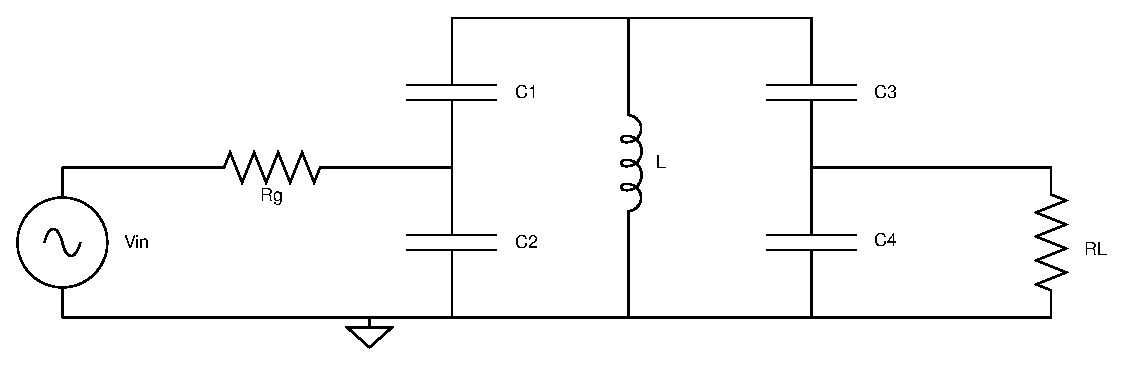
\includegraphics[width=0.7\textwidth]{./img/figura2.eps}
\caption{Circuito modificado.}
\label{fig:circuito2}
\end{figure}
\noindent De este circuito, se entiende que la capacitancia total resulta del paralelo entre dos partes en serie, en forma de expresión, se tiene lo siguiente:
\begin{equation*}
    C_T = \frac{C_1 C_2}{C_1 + C_2} + \frac{C_3 C_4}{C_3 + C_4}
\end{equation*}
Otra cosa que puede verse en el circuito es una especie de autotransformador. En donde podrían verse reflejadas las impedancias del generador y de la carga, y en donde las espiras de la máquina estática podrían ser representadas en este caso por los capacitores conectados, de esta forma. La parte a la que se hace referencia es la siguiente.
\begin{figure}[H]
\centering
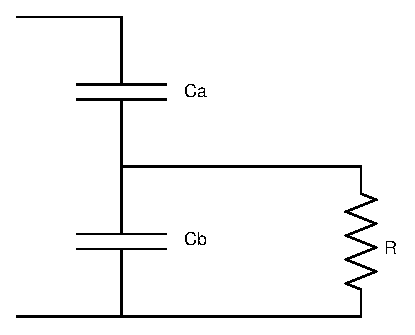
\includegraphics[width=0.3\textwidth]{./img/figura3.eps}
\caption{Circuito de reflexión de impedancia.}
\label{fig:circuito3}
\end{figure}
\noindent De las reflexiones, quedan expresadas las siguientes impedancias (el desarrollo de estas expresiones puede verse en el siguiente apartado del marco teórico):
\begin{equation*}
    R'_g = \left( 1 + \frac{C_2}{C_1} \right)^2 R_g
\end{equation*}
\begin{equation*}
    R'L = \left( 1 + \frac{C_4}{C_3} \right)^2 R_L
\end{equation*}
\noindent Con esos nuevos valores definidos, el circuito quedaría compuesto como el de la figura siguiente:
\begin{figure}[H]
\centering
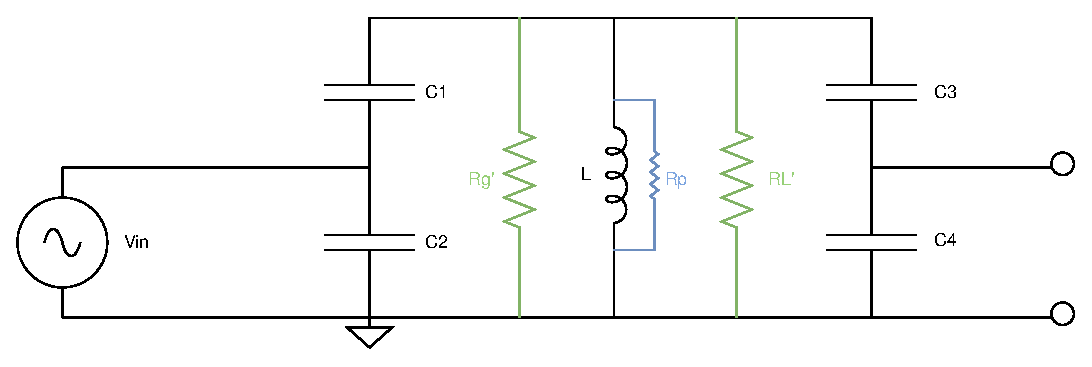
\includegraphics[width=0.7\textwidth]{./img/figura4.eps}
\caption{Circuito con impedancias reflejadas.}
\label{fig:circuito4}
\end{figure}
\noindent En este nuevo circuito, la impedancia total resulta del paralelo entre las reflejadas y la impedancia parásita de la bobina, es decir:
\begin{equation*}
    R_T = \left( \frac{1}{R'_g} + \frac{1}{R_p} + \frac{1}{R'_L}\right) ^{-1}
\end{equation*}
\noindent Con este circuito es posible sintonizar las resistencias reflejadas mediante la variación de las relaciones entre $C_1$ y $C_2$, o entre $C_3$ y $C_4$. 
Para el caso de desarrollo práctico abordado en este trabajo, se adaptan las impedancias de modo de obtener la máxima transferencia de energía, entonces, se plantea que:
\begin{equation*}
    R_T = 2 R_T // 2 R_T
\end{equation*}
\noindent En donde: 
\begin{equation*}
    R'_g = 2 R_T
\end{equation*}
\noindent Y, por otro lado:
\begin{equation*}
    R_p // R'_L = 2R_T
\end{equation*}
\noindent De la expresión del factor de potencia cargado, se puede obtener el ancho de banda deseado, fijando así el valor de la resistencia total.
\begin{equation*}
    X_L \cdot Q_c = R_T 
\end{equation*}
\noindent Para adaptar la impedancia de salida, se puede analizar el paralelo entre los resistores que representan la carga del sistema y la impedancia parásita de la bobina. Agrupando esos términos se puede lograr obtener lo mencionado anteriormente, luego de la explicación de la salida del análogo al \textit{“autotransformador de impedancias”}.
Finalmente, luego de este desarrollo, queda conformado un sistema de 4 ecuaciones no lineales, que servirán para el posterior diseño del inductor y circuito resonante. El sistema en cuestión es el siguiente:
\begin{equation*}
    \begin{cases}
        R'L = \left( 1 + \frac{C_3}{C_4} \right)^2 R_L \\
        \\
        R'_g = \left( 1 + \frac{C_2}{C_1} \right)^2 R_g \\
        \\
        \frac{C_1 C_2}{C_1 + C_2} = \frac{C_T}{2} \\
        \\
        \frac{C_3 C_4}{C_3 + C_4}= \frac{C_T}{2}
    \end{cases}
\end{equation*} 
%-------------------------------------------------------------------------%
\subsection{Condiciones para la reflexión de impedancias}
Para poder cumplir con la reflexión de impedancias de forma correcta, es necesario realizar una simplificación a modo de obtener la relación mencionada anteriormente. Para ello, se parte de un circuito mixto y se lo lleva a otro paralelo en forma equivalente. La transformación de circuitos que se pretende realizar se muestra a continuación.
\begin{figure}[H]
\centering
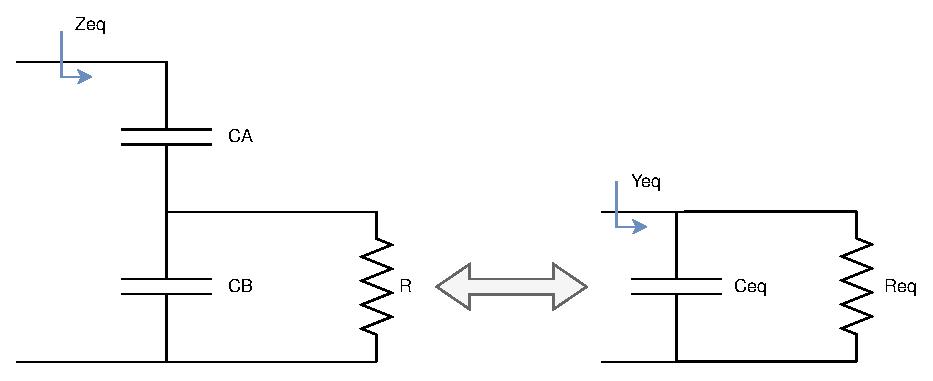
\includegraphics[width=0.7\textwidth]{./img/figura5.eps}
\caption{Circuitos equivalentes en reflexión de impedancias.}
\label{fig:circuito5}
\end{figure}
Primero que nada, se desarrolla la expresión de la impedancia equivalente $Z_{eq}$. Para ello, por simplicidad en el cálculo, se asume que:
\begin{equation*}
    X_C = -j \frac{1}{\omega C}
\end{equation*}
\noindent Hecha la aclaración, se comienza con el desarrollo:
\begin{align*}
    Z_{eq} &= XC_A + XC_B // R = XC_A + \frac{XC_B \cdot R}{XC_B + R} = \frac{XC_A XC_B + XC_A \cdot R + XC_B \cdot R}{R + XC_B} \\
    &= \frac{XC_A + \frac{XC_A}{XC_B}\cdot R + R}{\frac{R}{XC_B} + 1} = \frac{-j \frac{1}{\omega C_A} + \frac{CB}{CA}\cdot R + R}{1 + j R\omega C_B} = \frac{R \left( 1 + \frac{C_B}{C_A} \right) - j \frac{1}{\omega C_A}}{1 + jR\omega C_B}
\end{align*}
\noindent Luego, puede verse que si se quiere lograr un circuito equivalente que sea modelado completamente en paralelo, se podría trabajar con admitancias, ya que muestran una mayor facilidad de operación.
\begin{align*}
    Y_{eq} &= \frac{1}{Z_eq} = \frac{1 + jR\omega C_B}{R \left( 1 + \frac{C_B}{C_A} \right) - j \frac{1}{\omega C_A}} \cdot \frac{R \left( 1 + \frac{C_B}{C_A} \right) + j \frac{1}{\omega C_A}}{R \left( 1 + \frac{C_B}{C_A} \right) + j \frac{1}{\omega C_A}} \\
    &= \frac{R \left( 1 + \frac{C_B}{C_A} \right) + j \frac{1}{\omega C_A} + j R^2\omega C_B \left( 1 + \frac{C_B}{C_A}\right) - R \cdot \frac{C_B}{C_A}}{R^2 \left( 1 + \frac{C_B}{C_A} \right)^2 + \frac{1}{\omega^2 C_A^2}} \\
    &= \frac{R + j R^2\omega C_B \left( 1 + \frac{C_B}{C_A} \right) \cdot \frac{1}{\omega C_A}}{R^2 \left( 1 + \frac{C_B}{C_A} \right)^2 + \frac{1}{\omega^2 C_A^2}}
\end{align*}
\noindent De allí, se extrae la parte real de esa impedancia, para poder modelar la resistencia equivalente, siendo esta como se muestra a continuación.
\begin{equation*}
    R_{eq} = \frac{R^2 \left( 1 + \frac{C_B}{C_A} \right)^2 + \frac{1}{\omega^2 C_A^2}}{R} = R \left( 1 + \frac{C_B}{C_A} \right)^2 + \frac{1}{R\omega^2C_A^2}
\end{equation*}
\noindent Según las expresiones mostradas que muestran la reflexión de impedancias, el segundo término de este cálculo realizado no debería aparecer, es por eso que se busca que sea despreciable. Para lograr eso, se debe hacer que el denominador sea mucho mayor que 1, es decir:
\begin{equation*}
    R\omega ^2 C_A^2 >> 1
\end{equation*}
\noindent Para que ello se cumpla, teniendo en cuenta los órdenes de magnitud de frecuencia utilizados en los circuitos desarrollados, es necesario que el capacitor tenga un valor superior aproximadamente a los $100 pF$.
%-------------------------------------------------------------------------%
\subsection{Redes L}
Se parte del teorema de la máxima transferencia de energía, que deduce que para una carga caracterizada por una cierta impedancia $Z_L$, la forma de que reciba la máxima potencia útil del generador que la alimenta es bajo la condición de que:
\begin{equation*}
    Z_L = Z_g^*
\end{equation*}
\noindent Es decir, que es necesario que la impedancia de la carga sea el complejo conjugado de la impedancia presentada por el generador a su salida. En el caso de que ambas impedancias sean puramente resistivas, es necesario que sean iguales, es decir:
\begin{equation*}
    R_L = R_g
\end{equation*}
Las condiciones anteriores son difíciles de cumplir en la práctica, es por eso que es necesario normalmente utilizar redes que proporcionen una adaptación de impedancias. En este desarrollo se trabajará con impedancias reales, es decir, puramente resistivas. Con esta simplificación es posible utilizar la teoría de síntesis de filtros.

Se tienen diferentes topologías de la red L de acoplamiento, en la figura siguiente se muestran 4 diferentes, en donde:
\begin{itemize}
    \item Circuitos a) y b) son filtros pasa bajos.
    \item Circuitos c) y d) son filtros pasa altos.
\end{itemize}
\begin{figure}[H]
\centering
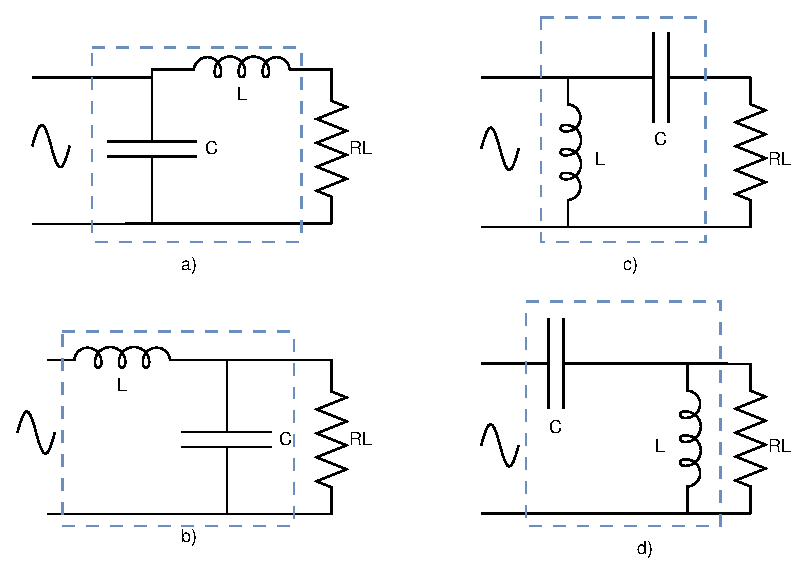
\includegraphics[width=0.7\textwidth]{./img/figura6.eps}
\caption{Topologías redes de acoplamiento L.}
\label{fig:circuito6}
\end{figure}
\noindent Como resultado de alguno de los circuitos anteriores se obtiene un circuito resonante serie, es decir, que tiene una impedancia muy baja en la frecuencia de resonancia, definida como $f_o$.  Se muestra a continuación, para el caso más común, es decir, impedancia de carga mayor a la de salida del generador. 
\begin{figure}[H]
\centering
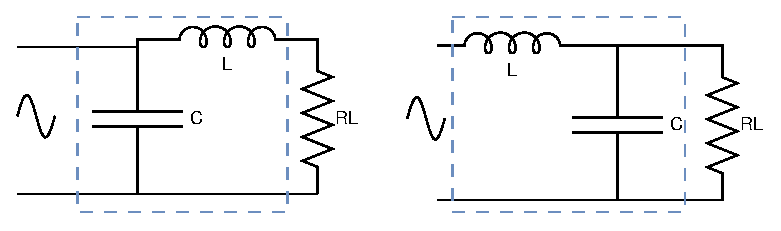
\includegraphics[width=0.7\textwidth]{./img/figura7.eps}
\caption{Redes de acoplamiento L.}
\label{fig:circuito7}
\end{figure}
\newpage
\noindent Las ecuaciones de diseño de la red de la izquierda son las siguientes:
\begin{equation*}
    X_L = \sqrt{R_gR_L - R_L^2}
\end{equation*}
\begin{equation*}
    Q = \sqrt{\frac{R_L}{R_g} - 1}
\end{equation*}
\begin{equation*}
    X_C = \frac{R_gR_L}{X_L}
\end{equation*}
\noindent Para ambas topologías, la frecuencia de resonancia viene dada por:
\begin{equation*}
    f_0 = \frac{1}{2\pi \sqrt{LC}}
\end{equation*}
\noindent De las ecuaciones de diseño mostradas arriba, es posible obtener una impedancia de carga equivalente a la de salida del generador, por lo que se estaría cumpliendo el teorema de la máxima transferencia de energía.
Este tipo de acoplamiento es utilizado en las siguientes aplicaciones:
\begin{itemize}
    \item Filtros pasa bajos y pasa altos.
    \item Estabilización de sistemas de potencia.
    \item Filtros de ruido y supresión de interferencias.
    \item Resonadores y osciladores.
    \item Compensación de impedancias.
\end{itemize}
%-------------------------------------------------------------------------%
\subsection{Inductores con núcleo de aire (monocapa)}
Esta configuración es generalizada en circuitos electrónicos gracias a la constancia de su valor de inductancia, el rango de utilización va de 1.5 MHz a 200 MHz aproximadamente. 

Normalmente se trabaja con bobinas con ejes rectos, construidos con alambre macizo, bobinados en el aire, es decir, auto soportados, o sobre formas de material aislante (como pueden ser porcelanas, cerámicas, etc.) que tienen aristas para disminuir los puntos de contacto.

Este tipo de inductores puede considerarse como bobinas toroidales de eje rectificado, lo que hace que la longitud deje de ser infinita, apareciendo la necesidad de introducir un factor k de Nagaoka, menor que la unidad, que depende de las dimensiones geométricas de la bobina y se expresa en función del cociente entre diámetro interior y la longitud de esta.
\newpage
Se tiene un esquema como el visto a continuación.
\begin{figure}[H]
\centering
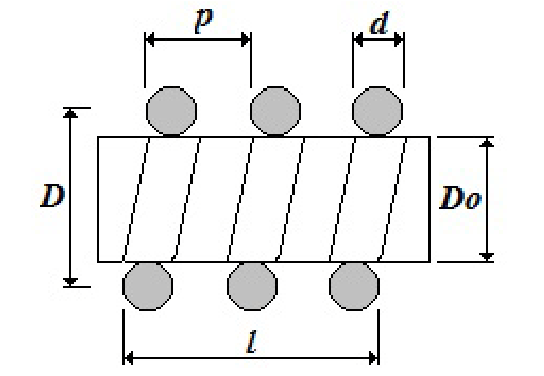
\includegraphics[width=0.4\textwidth]{./img/figura8.png}
\caption{Inductor con núcleo de aire, medidas importantes.}
\caption*{Fuente: Inductores con Núcleo de Aire, UTN Facultad Regional Mendoza.}
\label{fig:circuito8}
\end{figure}
\noindent En donde:
\begin{itemize}
    \item $D$: diámetro del inductor,
    \item $D_0$: diámetro de la forma,
    \item $d$: diámetro del conductor,
    \item $p$: paso,
    \item $N$: número total de espiras,
    \item $l$: longitud del inductor.
\end{itemize}
\subsubsection{Ventajas}
Como principales ventajas de este tipo de bobinados se puede señalar:
\begin{itemize}
    \item Su inductancia $L$ se puede calcular con buena aproximación.
    \item La capacidad parásita distribuida $C_d$ es mínima, ya que un extremo está separado del otro y la separación entre espiras puede hacerse grande.
    \item •	Los bobinados auto soportados tienen menos pérdidas, debido a que no existe el soporte aislante (forma).
    \item El efecto de proximidad es muy bajo, de modo que se pueden obtener $Q$ elevados y utilizarlos en alta frecuencia.
\end{itemize}
\subsubsection{Cálculo de la inductancia de un solenoide}
Si se tiene una longitud grande en comparación con el diámetro del inductor, se denomina lámina conductora, pero de sección rectangular, espesor y separación entre espiras prácticamente despreciable.
Si se tienen en cuenta las relaciones siguientes:
\begin{align*}
    L &= N \cdot \frac{\Phi}{I} \\
    \Phi &= B \cdot A \\
    B &= \mu \cdot H \\
    H &= N \frac{I}{l} \\
    \Phi &= \mu \cdot \frac{NI}{l} \cdot A \\
    L &= \mu \cdot \frac{N^2}{l} \cdot A \\
    \mu &= \mu_0 \cdot \mu_r    
\end{align*}
\noindent Siendo también que, en el vacío, para el sistema $MKS$:
\begin{equation*}
    \mu_0 = 4\pi 10^{-7} \left( \frac{Hy}{m} \right) = 4 \pi 10^{-9} \left( \frac{Hy}{cm} \right) = 4\pi 10^{-3} \left( \frac{\mu Hy}{cm} \right)
\end{equation*}
\noindent En donde, finalmente:
\begin{equation*}
    L = \frac{D^2 \cdot \pi^2 \cdot N^2}{l} \cdot 10^{-3} = 4 \cdot \frac{R^2 \cdot \pi^2 \cdot N^2 }{l} \cdot 10^{-3}
\end{equation*}
\indent Obteniéndose así el valor de la inductancia en $\mu Hy$ al utilizarse la longitud y el diámetro en centímetros.
Si se considera un solenoide completamente real, donde la longitud no es grande comparada con el diámetro, aparece el llamado efecto de borde y el campo magnético deja de ser perfectamente paralelo y homogéneo en el interior, por lo que las espiras exteriores no tienen una concatenación perfecta con las interiores.
\begin{figure}[H]
\centering
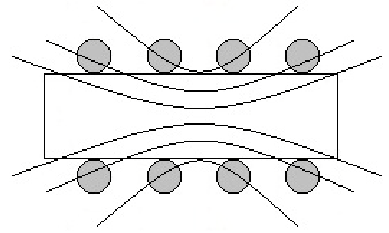
\includegraphics[width=0.4\textwidth]{./img/figura9.png}
\caption{Efecto borde en inductores con núcleo de aire.}
\caption*{Fuente: Inductores con Núcleo de Aire, UTN Facultad Regional Mendoza.}
\label{fig:circuito9}
\end{figure}
Nagaoka estudió en qué forma se altera la inductancia por el efecto de borde, adoptando así el llamado “factor de Nagaoka”. Dado que la mayoría de los inductores tienen longitudes comparables con sus diámetros, se puede obtener un factor de corrección, definido como:
\begin{equation*}
    k = \frac{1}{1 + 0.9 \cdot \frac{R}{l} - 2 \cdot 10^{-2} \cdot \left( \frac{R}{l} \right)^2}
\end{equation*}
\noindent El anterior factor asume que las espiras están juntas, si además se separan, es necesario aplicar otro factor de corrección, dado como:
\begin{equation*}
    \left[ 1 - \frac{l \cdot (A+ B)}{\pi \cdot R \cdot N \cdot k} \right]
\end{equation*}
\noindent Donde
\begin{equation*}
    A = 2.33Log\left(1.73 \frac{d}{p}\right)
\end{equation*}
\begin{equation*}
    B = 0.336\left( 1-\frac{2.5}{N}+ \frac{3.8}{N^2} \right)
\end{equation*}
\noindent Finalmente, la expresión de inductancia queda como:
\begin{equation*}
    L = k\cdot \frac{4R^2 \cdot \pi^2 \cdot N^2}{l}\cdot 10^{-3} \left[ 1 - \frac{l \cdot (A+ B)}{\pi \cdot R \cdot N \cdot k} \right]
\end{equation*}
Existe además otro factor $K$, que se usa para el proyecto de diseño de inductores, que viene tabulado y en formato de gráficas. Además de ese factor, aparece la relación entre las espiras y la longitud, expresada en \textit{“cantidad de espiras por unidad de longitud”}, en este caso, trabajando con centímetros (se denomina $Ns$). Finalmente, la fórmula de proyecto entonces queda dada por:
\begin{equation*}
    L = D^3 \cdot N_s^2 \cdot K \cdot 10^{-3} \quad [\mu Hy; cm]
\end{equation*}
\noindent Que es la fórmula utilizada para el diseño del inductor en este trabajo práctico.
%-------------------------------------------------------------------------%
\newpage
\section{Diseño del inductor}
Para diseñar el circuito resonador, se parte de las especificaciones de diseño brindadas en la clase práctica:
\begin{itemize}
    \item $f_0 = 13 MHz$,
    \item $Z_g = 50 \Omega$,
    \item $Z_L = 1 k\Omega$,
    \item $Q_c = 10$.
\end{itemize}
\noindent Con las anteriores, y, el sistema de ecuaciones mencionado en el marco teórico, puede apreciarse que existe una gran cantidad de grados de libertad para sintetizar el circuito, es por eso que se decide fijar algunos parámetros para facilitar el diseño.
\subsection{Consideraciones}
Atendiendo a lo mencionado anteriormente, los valores que se pretende mantener constantes en el diseño del inductor son:
\begin{itemize}
    \item \textbf{Diámetro del inductor}: se utiliza un valor cómodo para poder enrollar el conductor por sobre un material rígido.
    \item \textbf{Separación entre espiras}:  se la deja fija en la misma medida del diámetro del conductor, esto se define de forma arbitraria.
    \item \textbf{Diámetro del conductor}: se elige un diámetro intermedio entre uno muy chico (que no podría mantener fácilmente la forma) y uno muy grande (que dificulte el enrollar la bobina).
    \item \textbf{Paso}: depende de las magnitudes anteriores.
    \item \textbf{Frecuencia de resonancia}: fijada por los requisitos de diseño.
    \item \textbf{Ancho de banda}: fijado por los requisitos de diseño.
    \item \textbf{Factor de calidad cargado}: fijado por los requisitos de diseño.
    \item \textbf{Impedancia de entrada}:  fijada por los requisitos de diseño.
    \item \textbf{Impedancia de carga}: fijada por los requisitos de diseño.
\end{itemize}
\noindent Además de la fijación de los grados de libertad, lo siguiente a realizar fue decidir qué valor modificar para poder obtener diferentes posibilidades de inductor. En este caso, se optó por modificar el valor de la relación $l/D$ hasta encontrar un punto en que la cantidad de espiras no sea superior a $15$ ni menor a $6$, teniendo una cantidad redonda.

Otro valor a tener en cuenta fue el de los capacitores. Para ello, se diseñó a partir de los capacitores $2$ y $4$, para poder obtener a partir de esos capacitores los restantes en la relación, es decir $1$ y $3$. 
\subsection{Flujo del diseño}
El valor de la inductancia viene dado por:
\begin{equation*}
    L = D^3N_sk10^{-3} [\mu Hy]
\end{equation*}
\noindent En donde:
\begin{itemize}
    \item $D$ : diametro del inductor en $cm$,
    \item $N_s$: cantidad de espiras por $cm$,
    \item $k$: constante de proyecto.
\end{itemize}
\noindent Se decide que:
\begin{itemize}
    \item $D = 2 cm$,
    \item $S = 0.13 cm$,
    \item $d = 0.13 cm$,
    \item $p = 0.26 cm$.
\end{itemize}
\noindent La cantidad de vueltas por unidad de longitud resulta en:
\begin{equation*}
    N_s = \frac{1}{p} \cong 3.846 
\end{equation*}
\noindent Con esto en mente, puede mostrarse el siguiente gráfico, en donde se pueden apreciar las diferentes cantidades de vueltas para diferentes relaciones $l/D$. Se selecciona la cantidad de 10 espiras, que corresponde a la relación marcada en el gráfico.

\begin{figure}[H]
    \centering
    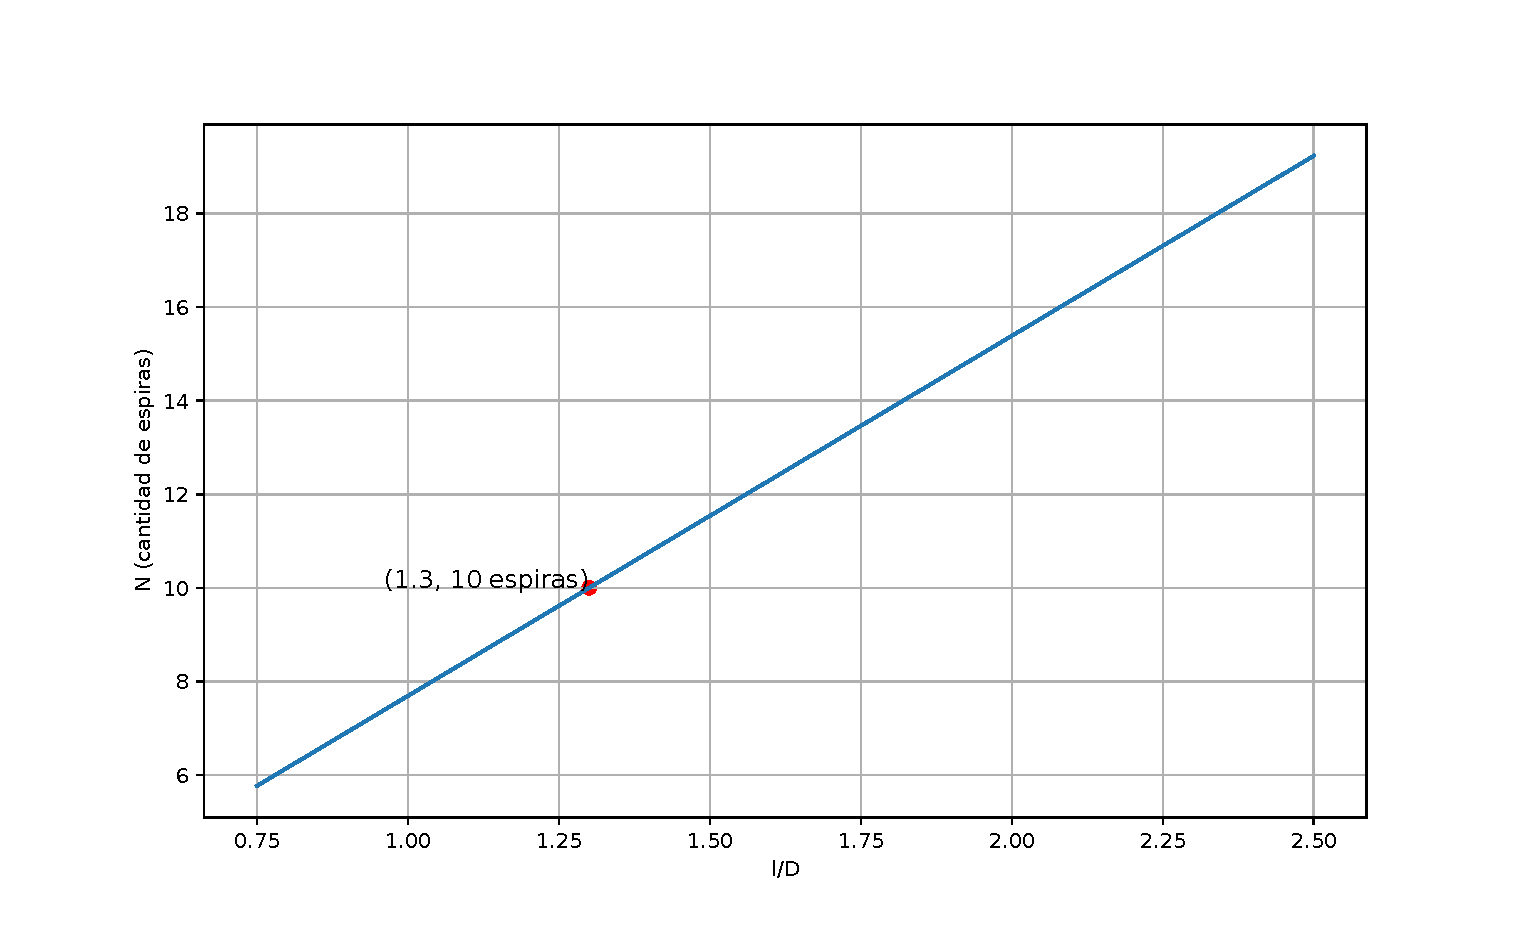
\includegraphics[width=0.8\textwidth]{./img/figura10.eps}
    \caption{Cantidad de espiras del inductor en función de la relación entre el diámetro y la longitud del bobinado.}
    \label{fig:circuito10}
\end{figure}

Para determinar la constante $k$ a utilizar en el proyecto de la bobina, se toman algunos puntos de la curva provista por la materia \textit{“Tecnología Electrónica”}, de modo de obtener una expresión mediante una interpolación polinómica, se aproximó a un polinomio de tercer grado. Se obtiene la siguiente expresión:
\begin{equation*}
    K = 0.88 \left( \frac{l}{D} \right)^3 - 30.3 \left( \frac{l}{D} \right)^2 + 42.77 \left( \frac{l}{D} \right) - 13.88
\end{equation*}
\noindent La curva interpolada, junto con los puntos puede verse en la siguiente figura.
\begin{figure}[H]
\centering
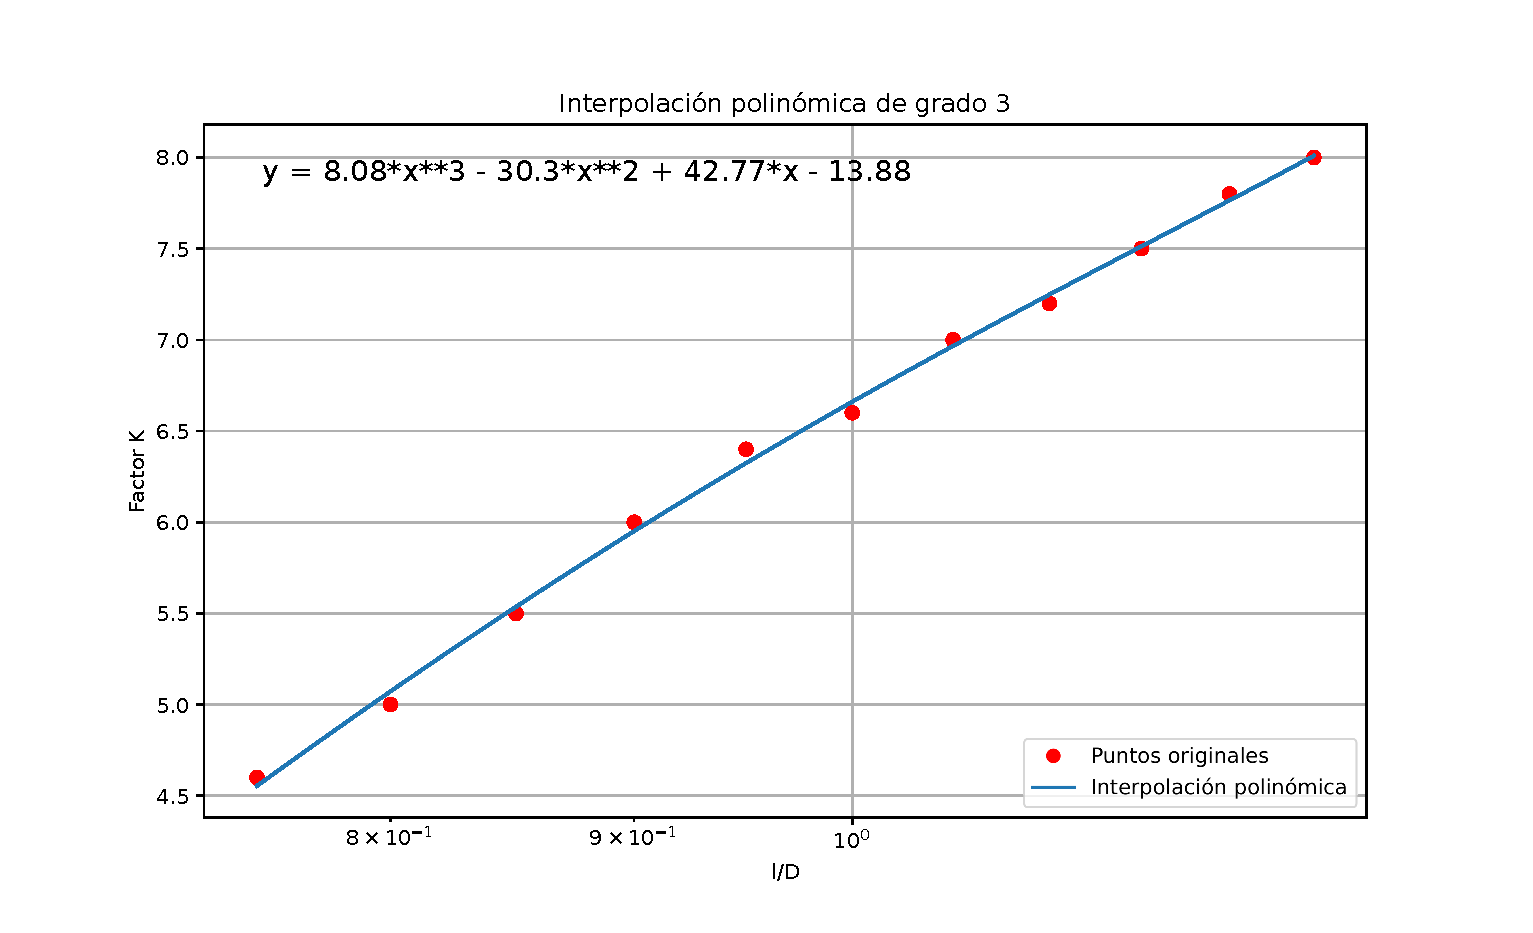
\includegraphics[width=0.85\textwidth]{./img/figura11.eps}
\caption{Interpolación polinómica del factor K.}
\label{fig:circuito11}
\end{figure}
\noindent Con el valor de K correspondiente al punto elegido de la curva, se procede a calcular la inductancia:
\begin{equation*}
    K = 8.266
\end{equation*}
\begin{equation*}
    L = 0.978196 \mu Hy 
\end{equation*}
\noindent Con ese valor de inductancia, para la frecuencia de resonancia se obtiene la siguiente reactancia inductiva:
\begin{equation*}
    X_L = 79.9 \Omega
\end{equation*}
\noindent Ahora, para el cálculo de la resistencia total del sistema, se usa el factor Q solicitado en la consigna, resultando así en:
\begin{equation*}
    R_T = \frac{f_0}{BW} 2\pi f_0L = 799 \Omega
\end{equation*}
\begin{equation*}
    Q_c = \frac{f_0}{BW} = 10
\end{equation*}
\noindent Para obtener el valor de la resistencia de pérdidas modelada en paralelo con la bobina, se parte del factor de calidad descargado, definido como:
\begin{equation*}
    Q_d = 8850 \frac{D \cdot l}{102l + 45D} \sqrt{f_0} = 467.14
\end{equation*}
\noindent De donde se despeja:
\begin{equation*}
    R_p = Q_d X_L = 37324.55 \Omega
\end{equation*}
\noindent Y, finalmente, los valores de resistores reflejados son:
\begin{equation*}
    R'_g = 2R_T = 1598 \Omega
\end{equation*}
\begin{equation*}
    2R_T = \frac{R'_L R_p}{R'_L + R_p} \Rightarrow R'_L = \frac{2R_T R_p}{R_p - 2R_T} = 1669.49 \Omega
\end{equation*}
\noindent Se muestran a continuación la dependencia de cada una de las magnitudes de resistencias mostradas últimamente, en función de la variable que se decidió manejar en el diseño, $l/D$.
\begin{figure}[H]
\centering
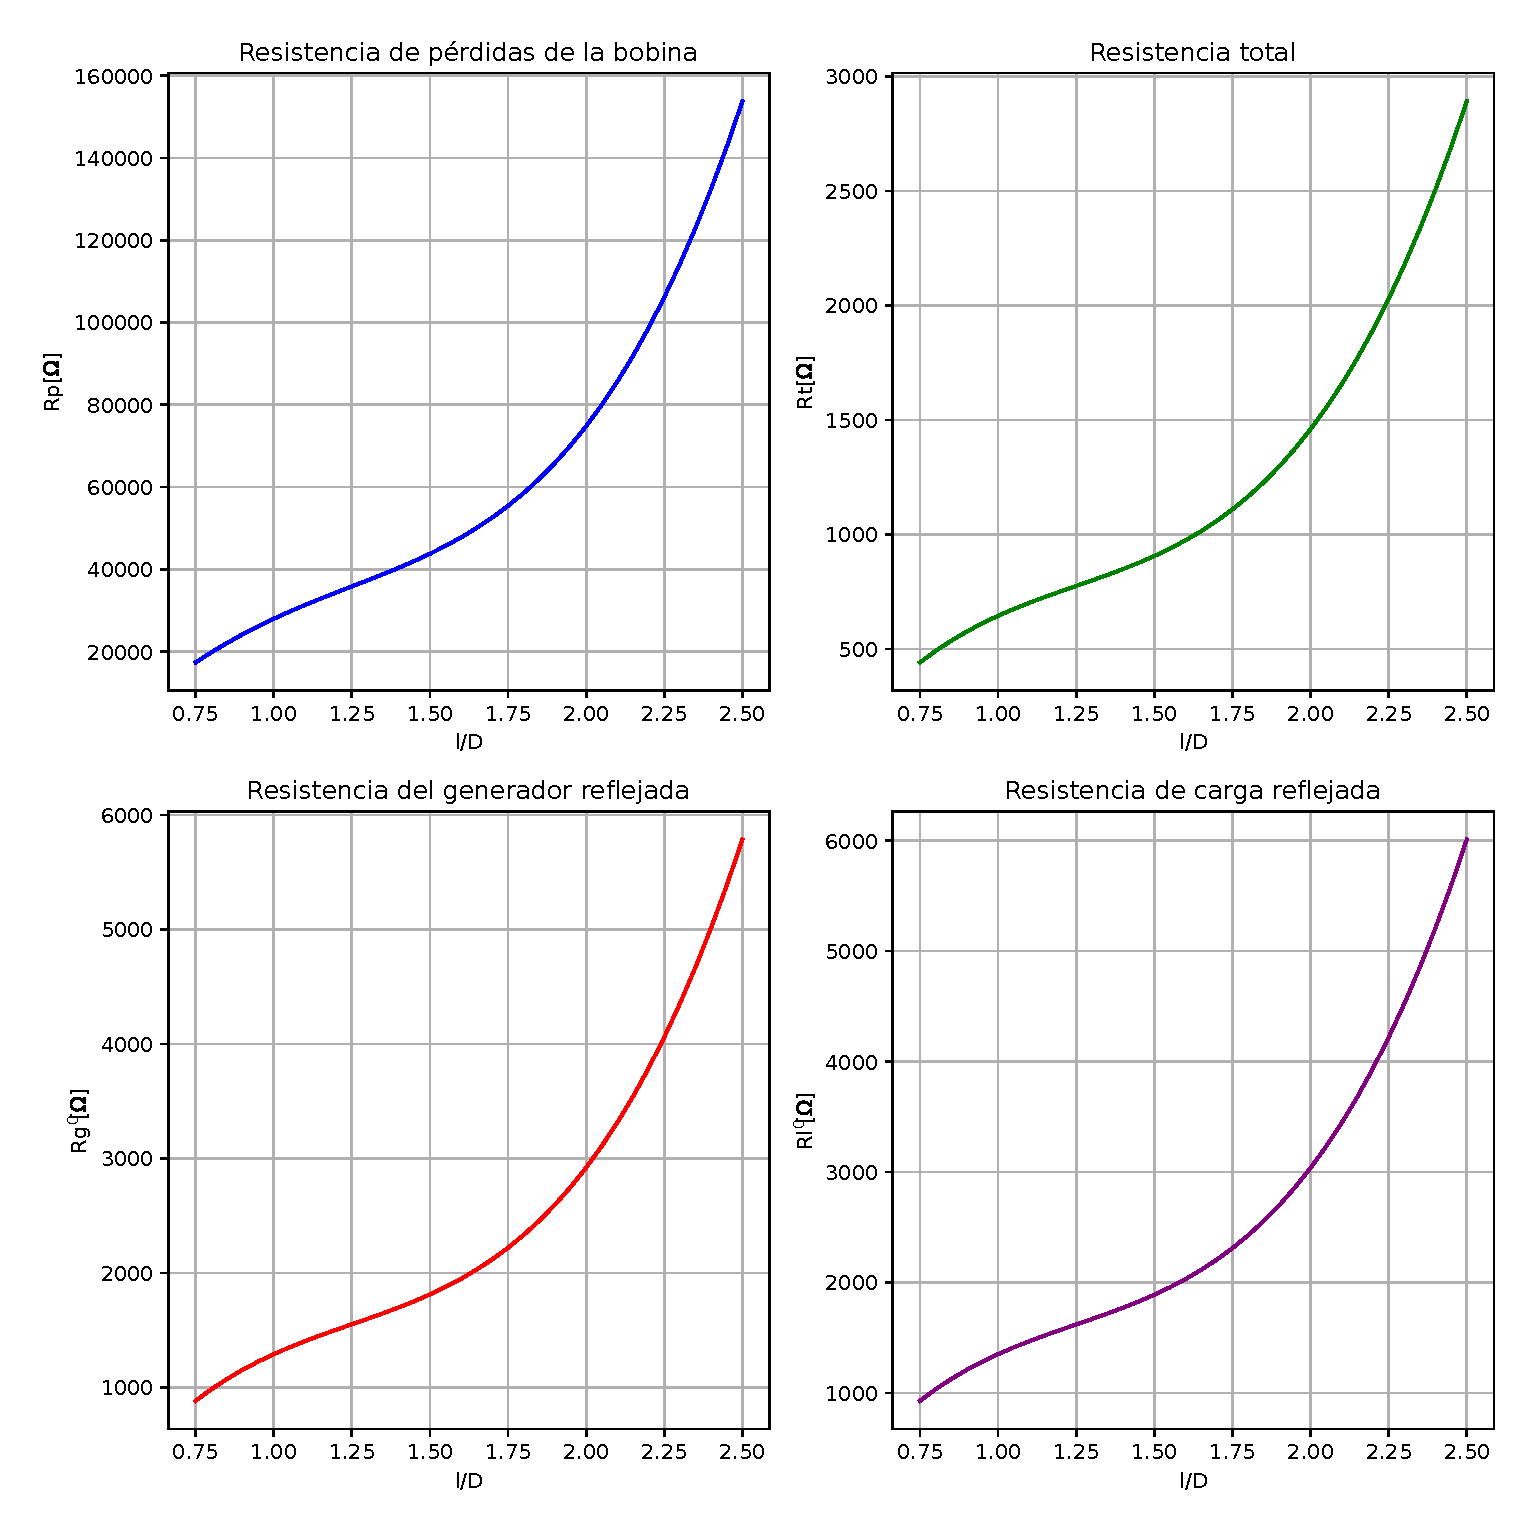
\includegraphics[width=0.7\textwidth]{./img/figura12.eps}
\caption{Variación de resistencias en función de la relación l/D.}
\label{fig:circuito12}
\end{figure}
\noindent La capacitancia total del sistema viene dada por el despeje de la ecuación que representa la frecuencia de resonancia del sistema, se tiene entonces:
\begin{equation*}
    C_T = \left( \frac{1}{2\pi f_0 \sqrt{L}} \right)^2 = 153.2 pF
\end{equation*}
\noindent Se obtienen las capacitancias a partir de la total, mencionada en el marco teórico como separada en 2 partes, cada parte siendo un grupo de 2 capacitores, que guardan una relación para el tema de reflexión de impedancias con la suerte de autotransformador obtenido. De esa forma, las expresiones que se usan para las capacitancias, junto con sus valores, son:
\begin{equation*}
    C_2 = \frac{C_t}{2} \left( 1 + \frac{C_2}{C_1} \right) = \frac{C_T}{2} \sqrt{\frac{2R_t}{R_g}} = 433.1 pF
\end{equation*}
\begin{equation*}
    C_1 = \frac{C_2}{\sqrt{\frac{R'_g}{R_g}-1}} = 77.8 pF
\end{equation*}
\begin{equation*}
    C_4 = \frac{C_T}{2} \left( 1 + \frac{C_4}{C_3} \right) = \frac{C_T}{2} \sqrt{\frac{2R_tR_p}{R_L(R_p - 2R_T)}}  = 99 pF
\end{equation*}
\begin{equation*}
    C_3 = \frac{C_4}{\sqrt{\frac{R'_L}{R_L}}- 1} = 338.9 pF
\end{equation*}
A modo de ilustración, se agregan las curvas resultantes de los capacitores del sistema:
\begin{figure}[H]
\centering
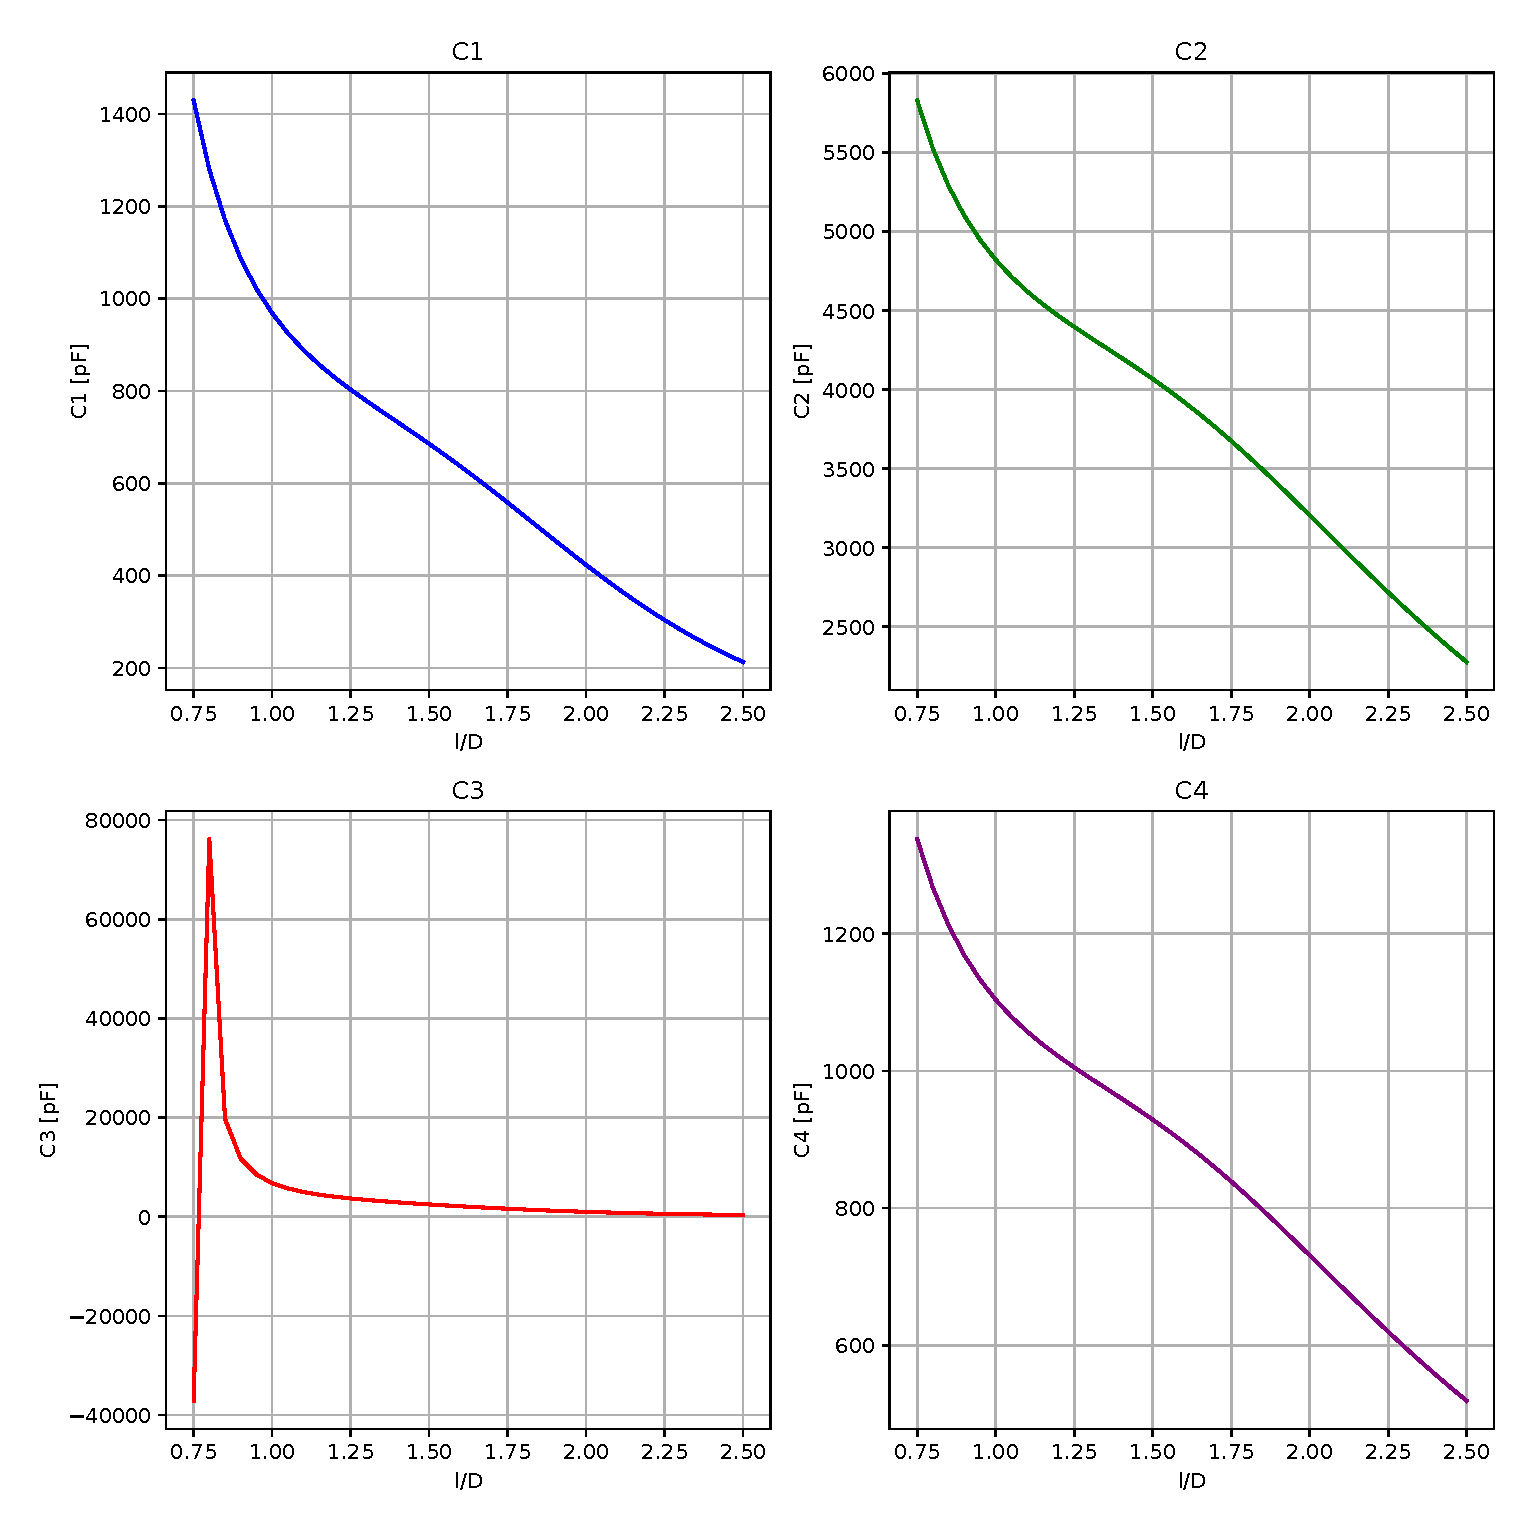
\includegraphics[width=0.7\textwidth]{./img/figura13.eps}
\caption{Evolución de la magnitud de los capacitores individuales en función de la relación $l/D$.}
\label{fig:circuito13}
\end{figure}
\newpage
\noindent Y la capacitancia total varía de acuerdo con:
\begin{figure}[H]
\centering
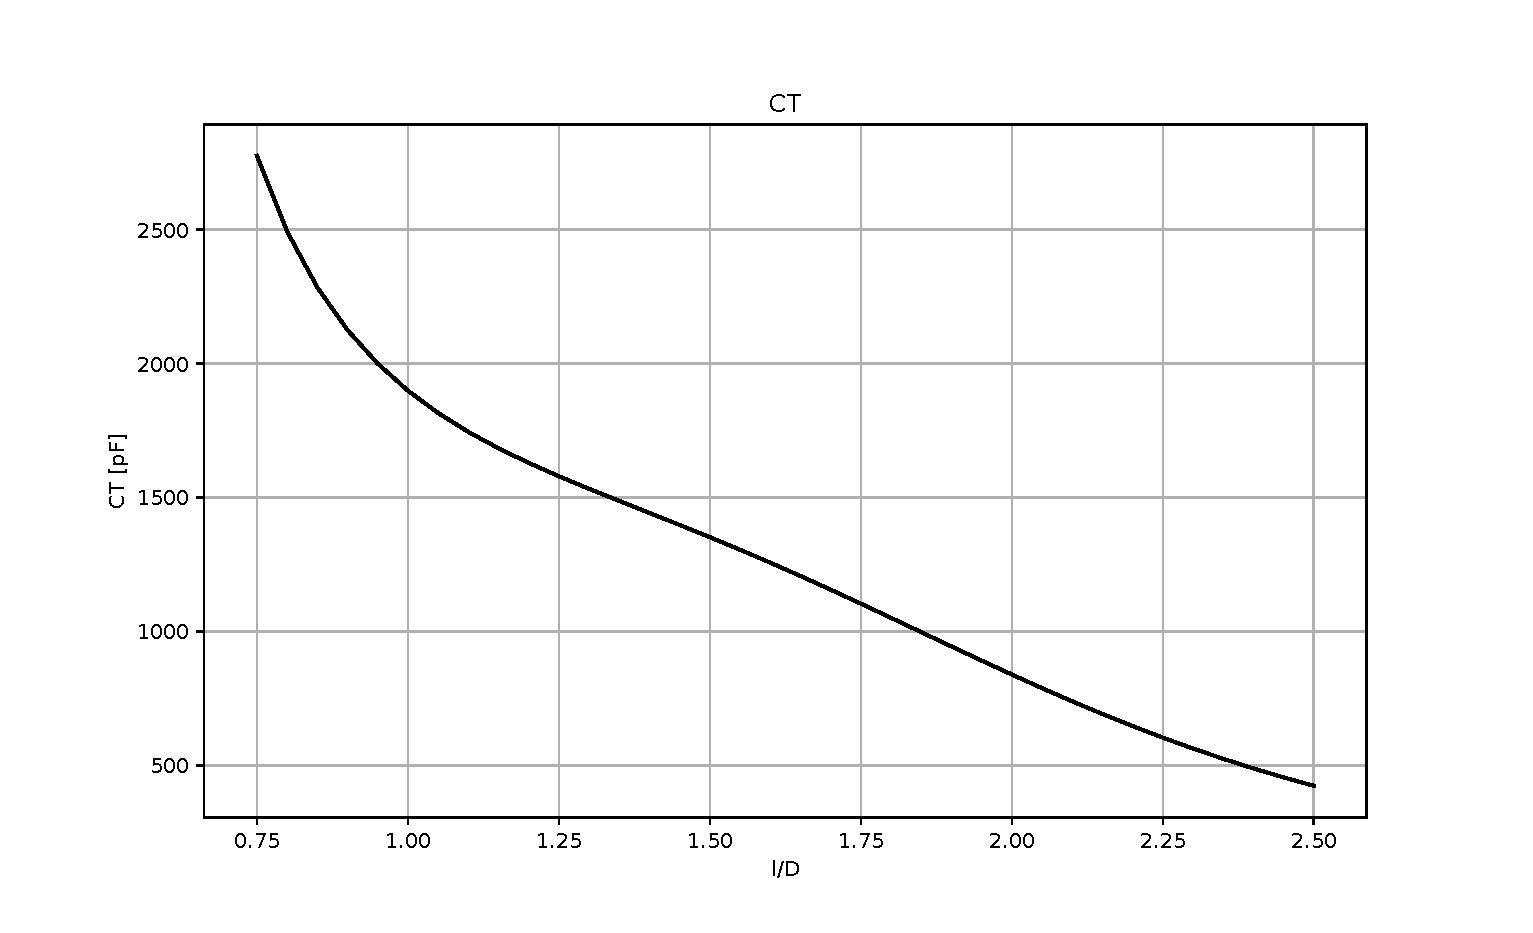
\includegraphics[width=0.7\textwidth]{./img/figura14.eps}
\caption{Capacitancia total en función de la relación $l/D$.}
\label{fig:circuito14}
\end{figure}
%-------------------------------------------------------------------------%
\newpage
\section{Simulación}
Para la simulación del sistema se utilizó el software LTSpice, de Analog Devices. En él se colocó el circuito que puede verse en la figura 15, y se realizó una corrida de análisis en frecuencia. 
\begin{figure}[H]
\centering
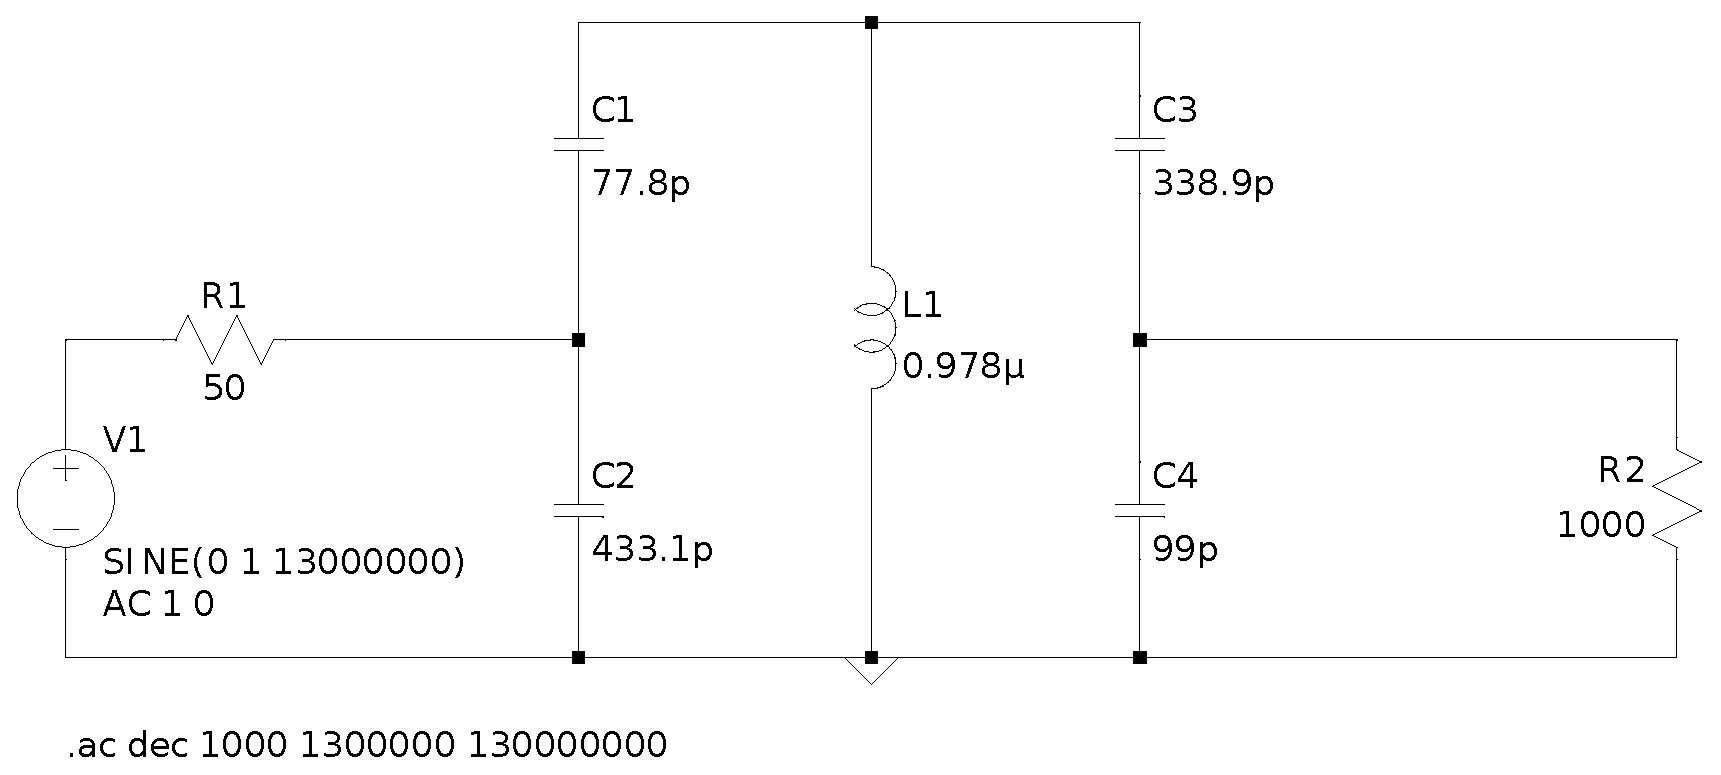
\includegraphics[width=1\textwidth]{./img/figura15.eps}
\caption{Circuito simulado en LTSpice.}
\label{fig:circuito15}
\end{figure}
\noindent Puede apreciarse también en la figura, que la directiva utilizada tiene como parámetros:
\begin{itemize}
\item Barrido en frecuencia por década.
\item 10000 puntos de resolución por década.
\item 1.3 MHz de frecuencia inicial.
\item 130 MHz de frecuencia final.
\end{itemize}
\noindent Se obtiene el siguiente diagrama de Bode de la corrida de la simulación.
\begin{figure}[H]
\centering
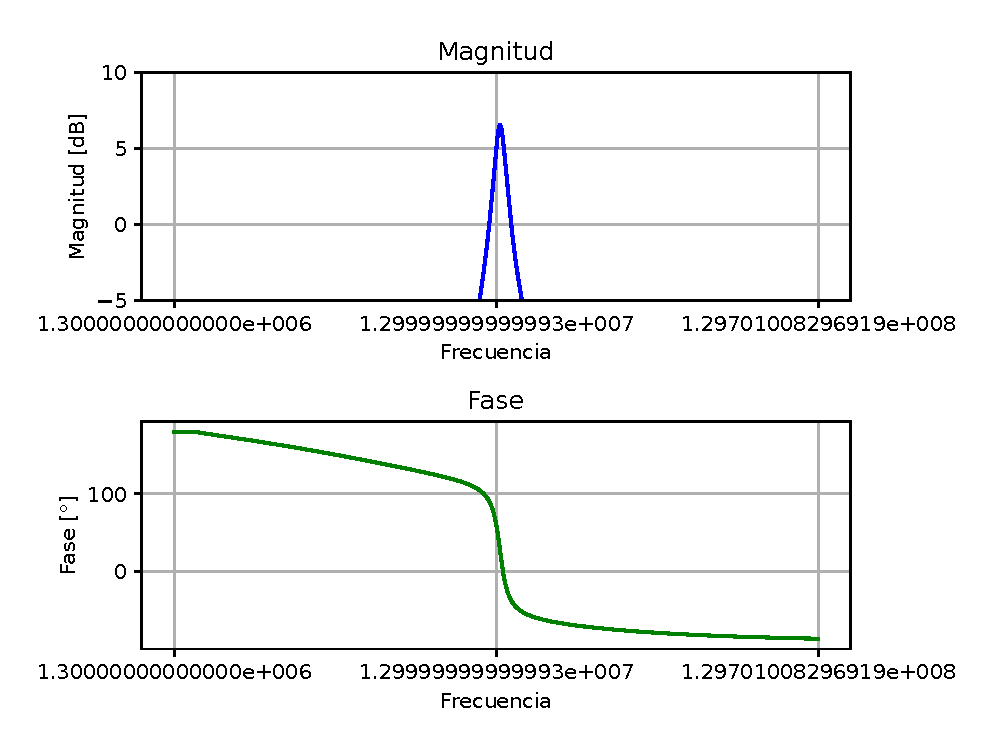
\includegraphics[width=1\textwidth]{./img/figura16.eps}
\caption{Diagrama de Bode de la respuesta del circuito diseñado.}
\label{fig:circuito16}
\end{figure}
\noindent Para encontrar el ancho de banda, se utilizó la herramienta de cursor de LTSpice, logrando así encontrar los siguientes datos.
\begin{figure}[H]
\centering
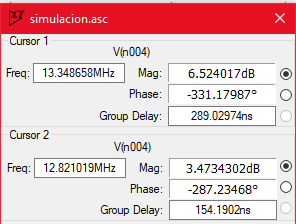
\includegraphics[width=0.35\textwidth]{./img/figura17.png}
\caption{Frecuencia menor de caída de 3dB.}
\label{fig:circuito17}
\end{figure}
\begin{figure}[H]
\centering
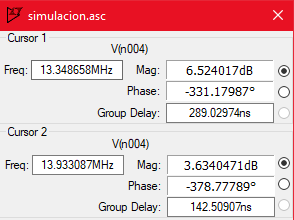
\includegraphics[width=0.35\textwidth]{./img/figura18.png}
\caption{Frecuencia mayor de caída de 3dB.}
\label{fig:circuito18}
\end{figure}
\noindent De donde resulta un ancho de banda de $1.11 MHz$, similar al de $1.3 MHz$ solicitado en los requisitos de diseño. Con este ancho de banda, junto con la frecuencia de resonancia, se obtiene un valor de factor de calidad cargado de $Q=\frac{13.34}{1.11}=12.01$.
%-------------------------------------------------------------------------%
\newpage
\section{Montaje}
En cuanto a los componentes utilizados para el montaje del circuito, se trabajó con lo siguiente:
\begin{itemize}
    \item Placa de cobre virgen, simple faz de 5x5 cm.
    \item Conectores BNC para PCB.
    \item Cable de cobre de 1.3 mm de diámetro.
    \item Capacitores de:    
        \begin{itemize}
            \item $5.6 pF$
            \item $330 pF$
            \item $3.3 pF$
            \item $100 pF$
            \item $390 pF$
            \item $33 pF$
            \item $68 pF$
            \item $2.2 pF$            
        \end{itemize}
\end{itemize}
\noindent Es importante notar, que, al usar valores de capacitancia normalizados, es dificil alcanzar exactamente el valor que se desea, por lo que se aclara a continuación, la combinación de capacitores en paralelo utilizada para lograr cada una de las capacitancias requeridas:
\begin{itemize}
    \item $C_1=(5.6+2.2+68)  pF=75.8 pF$
	\item $C_2=(33+390)  pF=423 pF$
	\item $C_3=(330+3.3+5.6)  pF=338.9 pF$
	\item $C_4=100 pF$
\end{itemize}
\noindent A su vez, los capacitores poseen una capacidad variable en un amplio rango, por la gran tolerancia con la que son comercializados, por lo que no es descabellado encontrar valores alejados de los esperados. Obviando este hecho, y por no contar con un instrumento de medición que pueda cuantificar la magnitud de capacitancia de cada componente, se los supone de la capacidad mencionada. Ahora, bajo este supuesto, la capacidad total del circuito resulta en:
\begin{align*}
    C_1 + C_2 &= 64.28 pF \\
    C_3 + C_4 &= 77.22 pF \\
    C_T &= 141.49 pF
\end{align*}
\subsection{Armado del inductor}
Para lograr que el bobinado tenga una separación entre espiras uniforme de acuerdo con lo diseñado, se diseñó un cilindro para luego ser impreso en 3D, que posee la rosca con el paso necesario.
\begin{figure}[H]
\centering
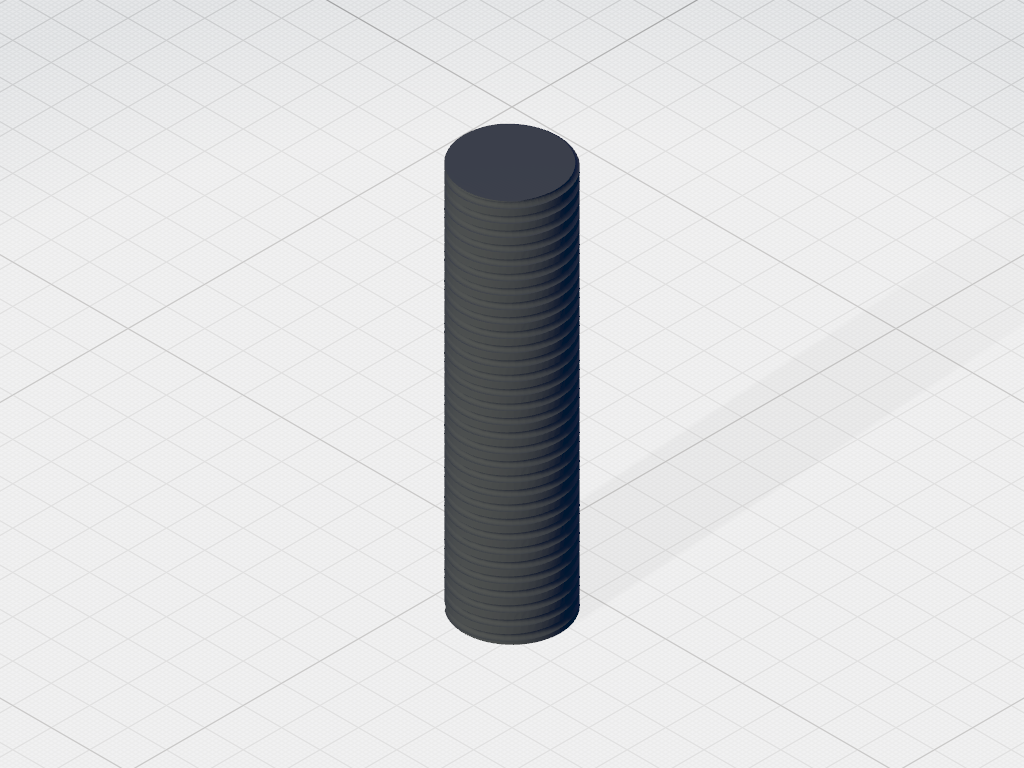
\includegraphics[width=0.5\textwidth]{./img/figura19.png}
\caption{Carretel para el correcto espaciamiento de las espiras en el bobinado.}
\label{fig:circuito19}
\end{figure}
\noindent Además, se imprimió en 3D otro carretel, hueco en este caso, que sirve para colocarlo en la bobina cuando no se esté usando el circuito. Este elemento es mucho más chico, y permite que las espiras mantengan la forma, es de fácil colocación y extracción, pues simplemente se trata de una rosca. Su forma se muestra en la figura siguiente.
\begin{figure}[H]
\centering
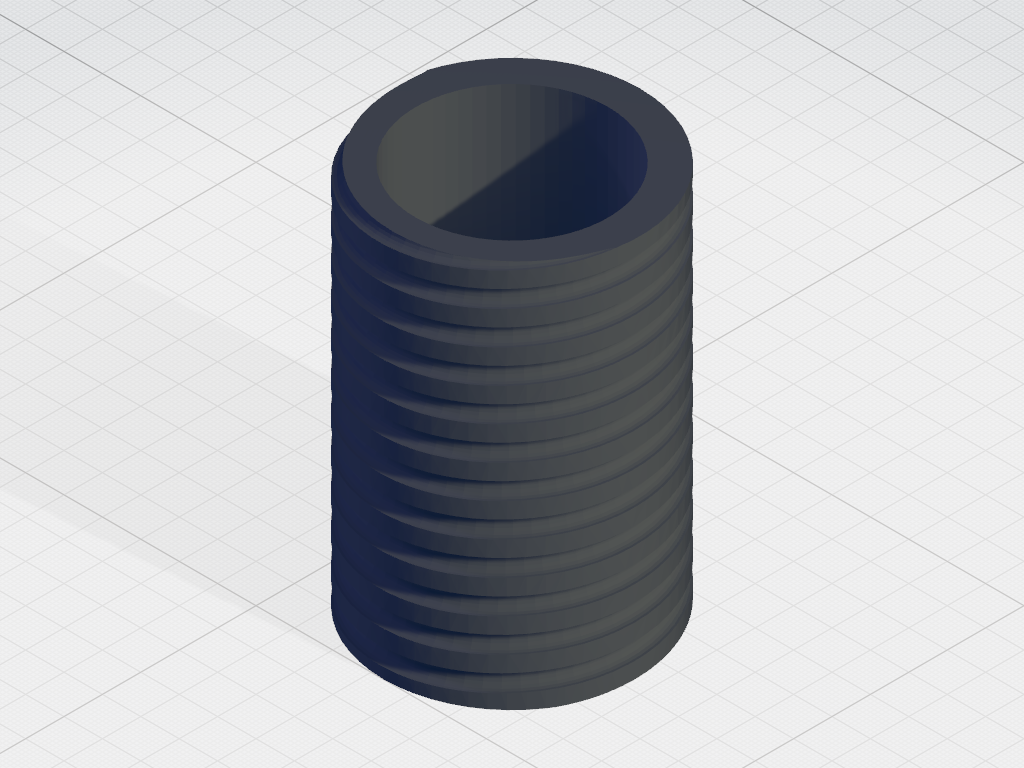
\includegraphics[width=0.5\textwidth]{./img/figura20.png}
\caption{Carretel hueco.}
\label{fig:circuito20}
\end{figure}
\subsection{Forma final}
El resultado del montaje del circuito es el siguiente.
\begin{figure}[H]
\centering
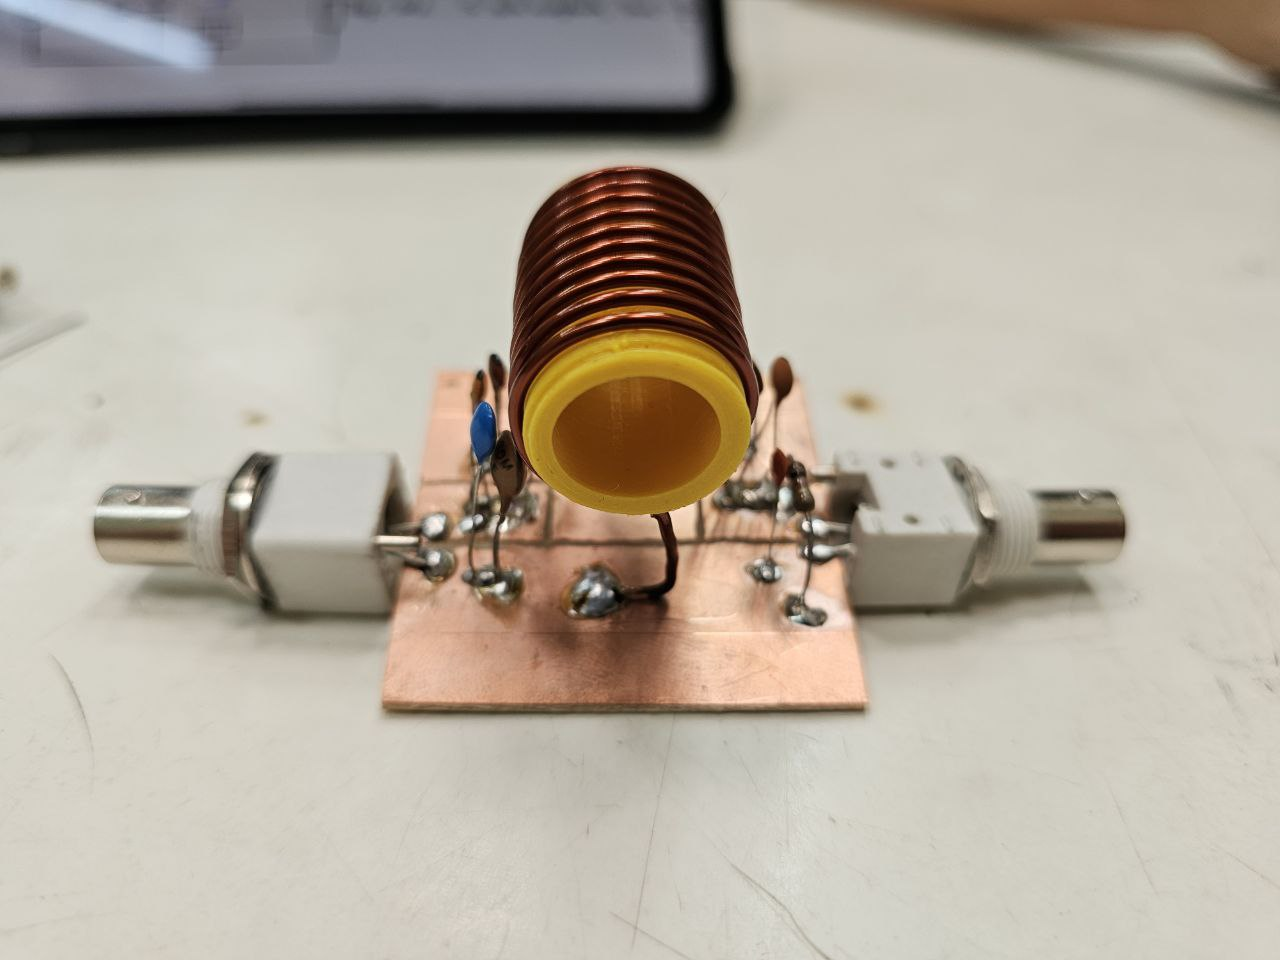
\includegraphics[width=0.7\textwidth]{./img/figura21.jpg}
\caption{Resultado final del montaje.}
\label{fig:circuito21}
\end{figure}
\newpage
\section{Mediciones}
\subsection{Procedimientos}
Cabe aclarar que, como los dispositivos que se utilizan para medir las magnitudes del circuito no son ideales, es decir, presentan impedancias y capacidades parásitas, el uso de estos termina modificando el circuito. Es por esta razón que, para obtener mediciones relevantes y confiables, es necesario utilizar algunas topologías o configuraciones especiales que contemplan las modificaciones que se le están realizando al circuito al momento de medir. Los resultados reales de los parámetros del circuito resultan de mediciones indirectas, pues, con lo obtenido en cada instrumento se realizan cálculos auxiliares que permiten cuantificar magnitudes reales. A continuación, se detallan los diferentes procedimientos utilizados para tomar mediciones.
\subsubsection{Medición de resistencia de pérdidas}
Para medir la resistencia de pérdidas de la bobina, se conecta en serie con el generador de RF una resistencia de pruebas, y se busca la resonancia del circuito. Una vez encontrada la frecuencia de resonancia, se toma la medición de la tensión con el osciloscopio, de forma de analizar el resistor de pérdidas a partir del divisor de tensión conformado. La topología usada se ve en la figura siguiente:
\begin{figure}[H]
\centering
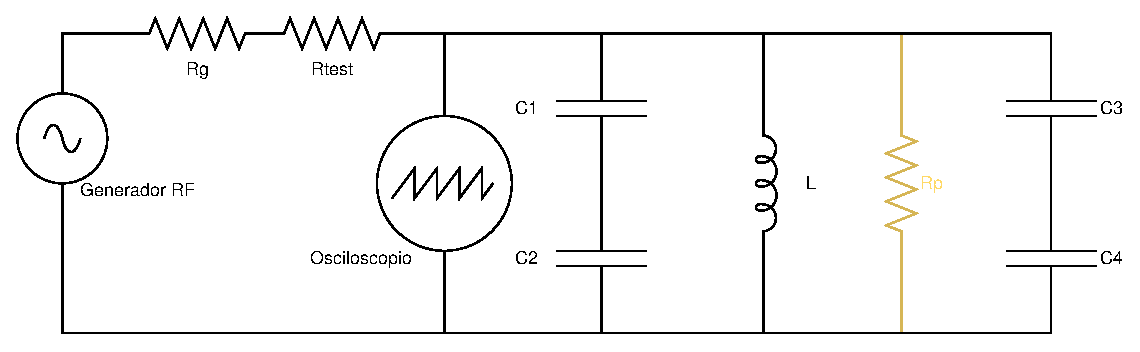
\includegraphics[width=0.7\textwidth]{./img/figura22.eps}
\caption{Topología del circuito para la medición de la resistencia de pérdidas.}
\label{fig:circuito22}
\end{figure}
\noindent Al trabajar en la frecuencia de resonancia, el circuito se reduce a lo siguiente.
\begin{figure}[H]
\centering
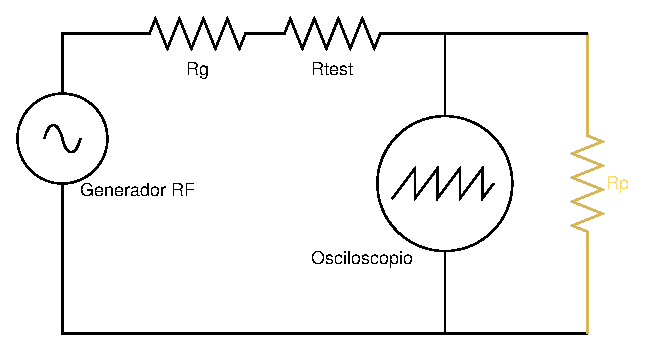
\includegraphics[width=0.5\textwidth]{./img/figura23.eps}
\caption{Circuito en resonancia para la medición de resistencia de pérdidas.}
\label{fig:circuito23}
\end{figure}
De la figura \ref{fig:circuito23} se puede obtener la resistencia de pérdidas mediante el siguiente cálculo:
\begin{equation*}
    R_p = \frac{V_{out} (R_g + R_{text})}{V_{in}- V_{out}}
\end{equation*}
\subsubsection{Medición de inductancia, frecuencia de resonancia y factor de calidad descargado}
Para la medición de la frecuencia de resonancia, es necesario utilizar la llamada “conexión a tope”, que resulta ser la topología de la figura \ref{fig:circuito22}.
\begin{figure}[H]
\centering
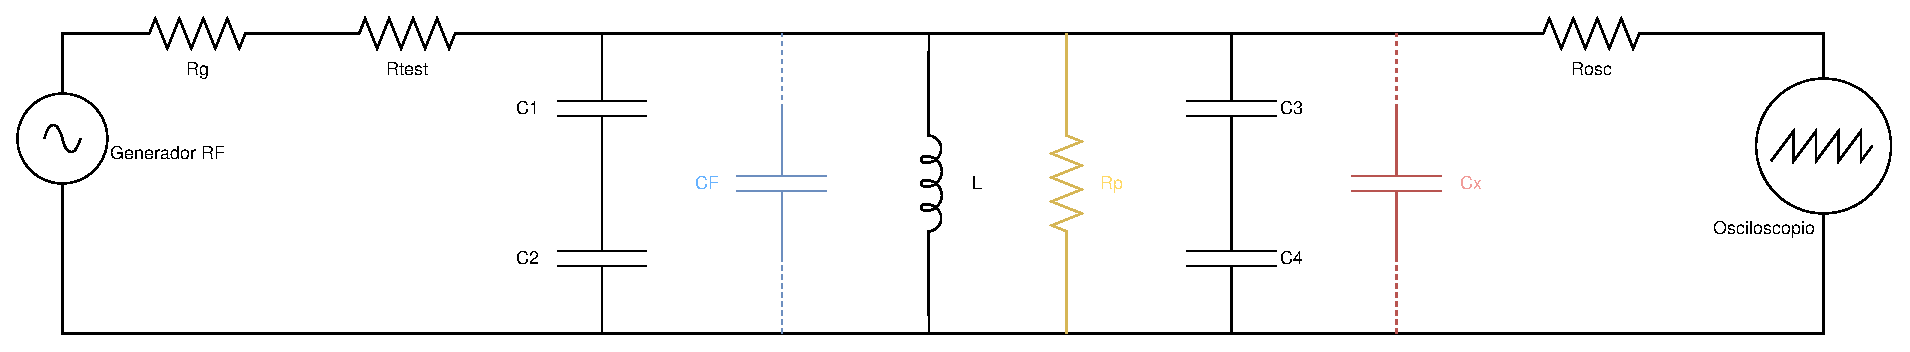
\includegraphics[width=0.9\textwidth]{./img/figura24.eps}
\caption{Conexión a tope para medir frecuencia de resonancia e inductancia.}
\label{fig:circuito24}
\end{figure}
\noindent En este circuito, se conecta una resistencia de test, que debe ser del orden de la resistencia de pérdidas del bobinado, de forma de evitar cortocircuitar el generador y permitir medir la tensión en resonancia. El $C_F$ es un capacitor físico, que sirve para tomar dos mediciones. 

En esta conexión:
\begin{equation*}
    C_{eq1} = C_T + C_x
\end{equation*}
En donde $C_x$ es la capacitancia del osciloscopio. El capacitor físico se conecta y desconecta, es por eso que en la figura \ref{fig:circuito22} se encuentra representado con línea de puntos. 

\noindent De esa forma se encuentran 2 frecuencias de resonancia distintas, definidas como:
\begin{equation*}
    R_{01} = \frac{1}{2\pi \sqrt{L(C_T+C_x)}} \quad R_{02} = \frac{1}{2\pi \sqrt{L(C_T+C_x+C_F)}}
\end{equation*}
\noindent Del cociente entre esas frecuencias puede despejarse el valor del capacitor parásito del osciloscopio.
\begin{equation*}
    \frac{R_{01}^2}{R_{02}^2} = \frac{C_T + C_x + C_f }{C_T + C_x}
\end{equation*}
\begin{equation*}
    C_x = \frac{C_T (R_{01}^2-R_{02}^2)+C_f R_{02}^2}{R_{01}^2-R_{02}^2}
\end{equation*}
\noindent Y, finalmente, se puede despejar el valor de la inductancia:
\begin{equation*}
    L = \left( \frac{1}{2\pi R_{01}}\right)^2 \cdot \frac{1}{C_T + C_x}
\end{equation*}
\noindent Con ese valor de inductancia se puede obtener la frecuencia de resonancia.
\begin{equation*}
    f_0 = \frac{1}{2\pi \sqrt{LC_T}}
\end{equation*}
\noindent Finalmente, puede obtenerse el valor del factor Q descargado, de la siguiente forma:
\begin{equation*}
    Q_d = \frac{R_p}{X_L} = \frac{R_p}{2\pi LF_0 (\text{medición Rp})}
\end{equation*}
\noindent Cabe aclarar que la frecuencia de resonancia que se debe usar es la obtenida en la medición de la resistencia de pérdidas de la bobina.
\subsubsection{Medición de impedancia de entrada}
Para la medición de impedancia de entrada se busca la resonancia en el siguiente circuito. Luego, una vez alcanzada esa condición, se mide la salida del generador de RF cargado y descargado con el osciloscopio. 
\begin{figure}[H]
\centering
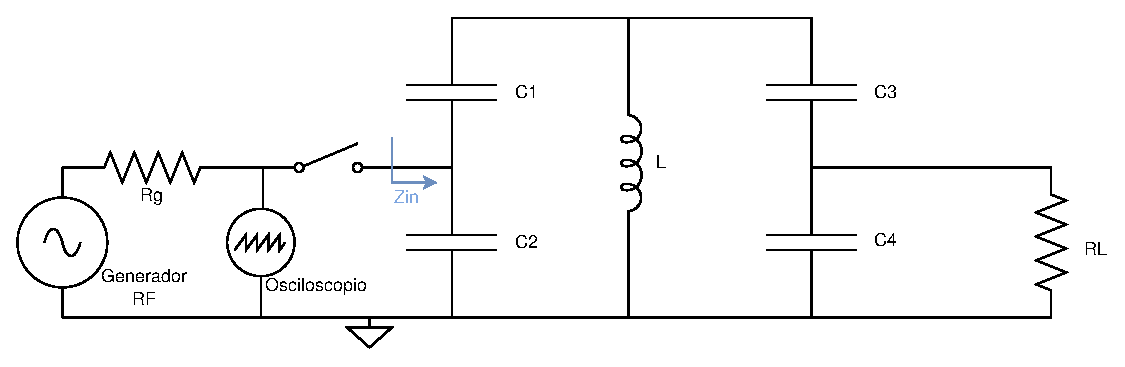
\includegraphics[width=0.9\textwidth]{./img/figura25.eps}
\caption{Circuito para la medición de impedancia de entrada.}
\label{fig:circuito25}
\end{figure}
\noindent De la medición, resulta la siguiente expresión:
\begin{equation*}
    Z_{in} = \frac{R_g}{\left( \frac{V_d}{V_c} - 1 \right)}
\end{equation*}
\noindent En donde:
\begin{itemize}
    \item $V_d$: tensión de salida del generador descargado.
    \item $V_c$: tensión de salida del generador cargado.
\end{itemize}
\subsubsection{Medición de impedancia de salida}
La medición de la impedancia de salida es similar a la de la medición de entrada (encontrando también una frecuencia de resonancia para cancelar el término imaginario de la expresión de la impedancia), solo que esta vez se trabaja con salida cargada y descargada, como puede apreciarse claramente en la figura a continuación, en donde se tiene un switch.
\begin{figure}[H]
\centering
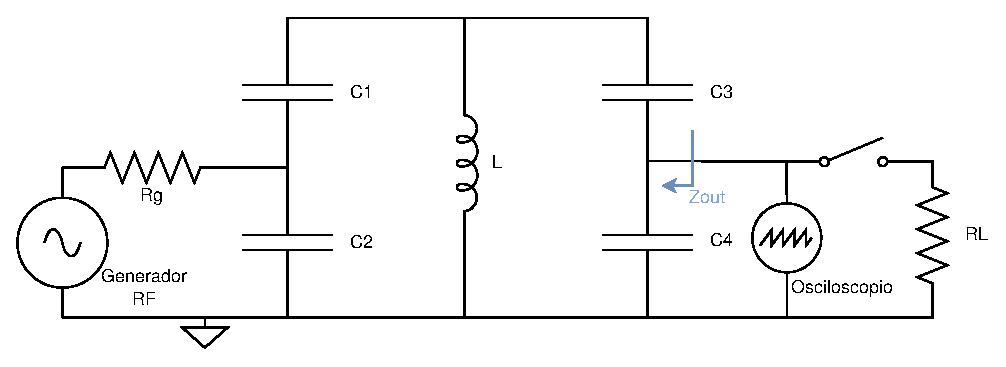
\includegraphics[width=0.9\textwidth]{./img/figura26.eps}
\caption{Circuito para la medición de impedancia de salida.}
\label{fig:circuito26}
\end{figure}
\noindent La expresión para el cálculo de la impedancia es:
\begin{equation*}
    Z_{out} = R_L \left( \frac{V_d}{V_c} - 1 \right)
\end{equation*}
\noindent En donde:
\begin{itemize}
    \item $V_d$: tensión de salida del generador descargado.
    \item $V_c$: tensión de salida del generador cargado.
\end{itemize}
\subsubsection{Medición de ancho de banda}
Para medir el ancho de banda del circuito se utiliza la siguiente configuración.
\begin{figure}[H]
\centering
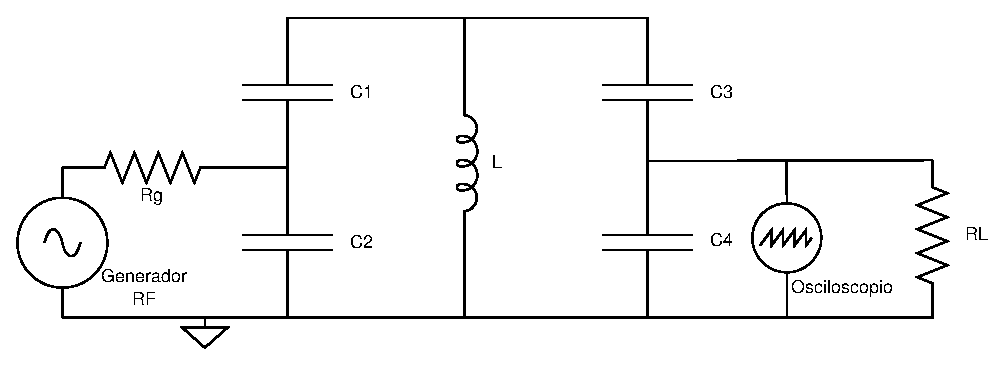
\includegraphics[width=0.9\textwidth]{./img/figura27.eps}
\caption{Circuito para la medición del ancho de banda.}
\label{fig:circuito27}
\end{figure}
Se busca la frecuencia de resonancia de este circuito, es decir, en donde la tensión de salida es máxima, ese valor es tabulado como $\widehat{V}$ Luego se buscan frecuencias superiores a inferiores a esa $f_o$ que disminuyan la salida en $3 dB$, es decir, se reduzcan en $\sqrt{2}$ veces. Con esto, se obtiene la diferencia entre esas frecuencias $f_1$ y $f_2$ y ese es el ancho de banda. Se debería poder obtener algo como lo mostrado en el siguiente gráfico (obtenido de \href{https://es.wikipedia.org/wiki/Filtro_paso_banda}{Wikipedia}).
\begin{figure}[H]
\centering
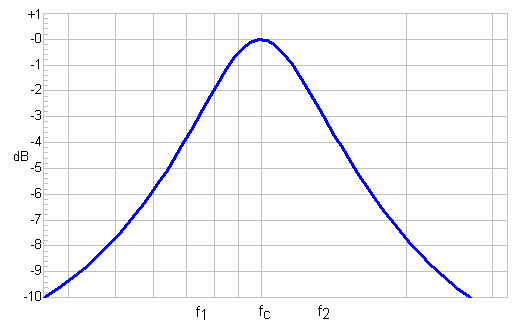
\includegraphics[width=0.6\textwidth]{./img/figura28.png}
\caption{Respuesta en frecuencia de un filtro pasa banda.}
\label{fig:circuito28}
\end{figure}
\subsection{Instrumentos}
Los instrumentos utilizados para las mediciones son los siguientes:
\begin{itemize}
    \item Generador de funciones GW Instek AFG-2125 (código GFA02).
    \item Osciloscopio Keysight DSO1052B (código OSC64).
\end{itemize}
\noindent Para poder monitorear la tensión de salida del generador en todo momento se utilizó una punta de prueba T-BNC.
\begin{figure}[H]
\centering
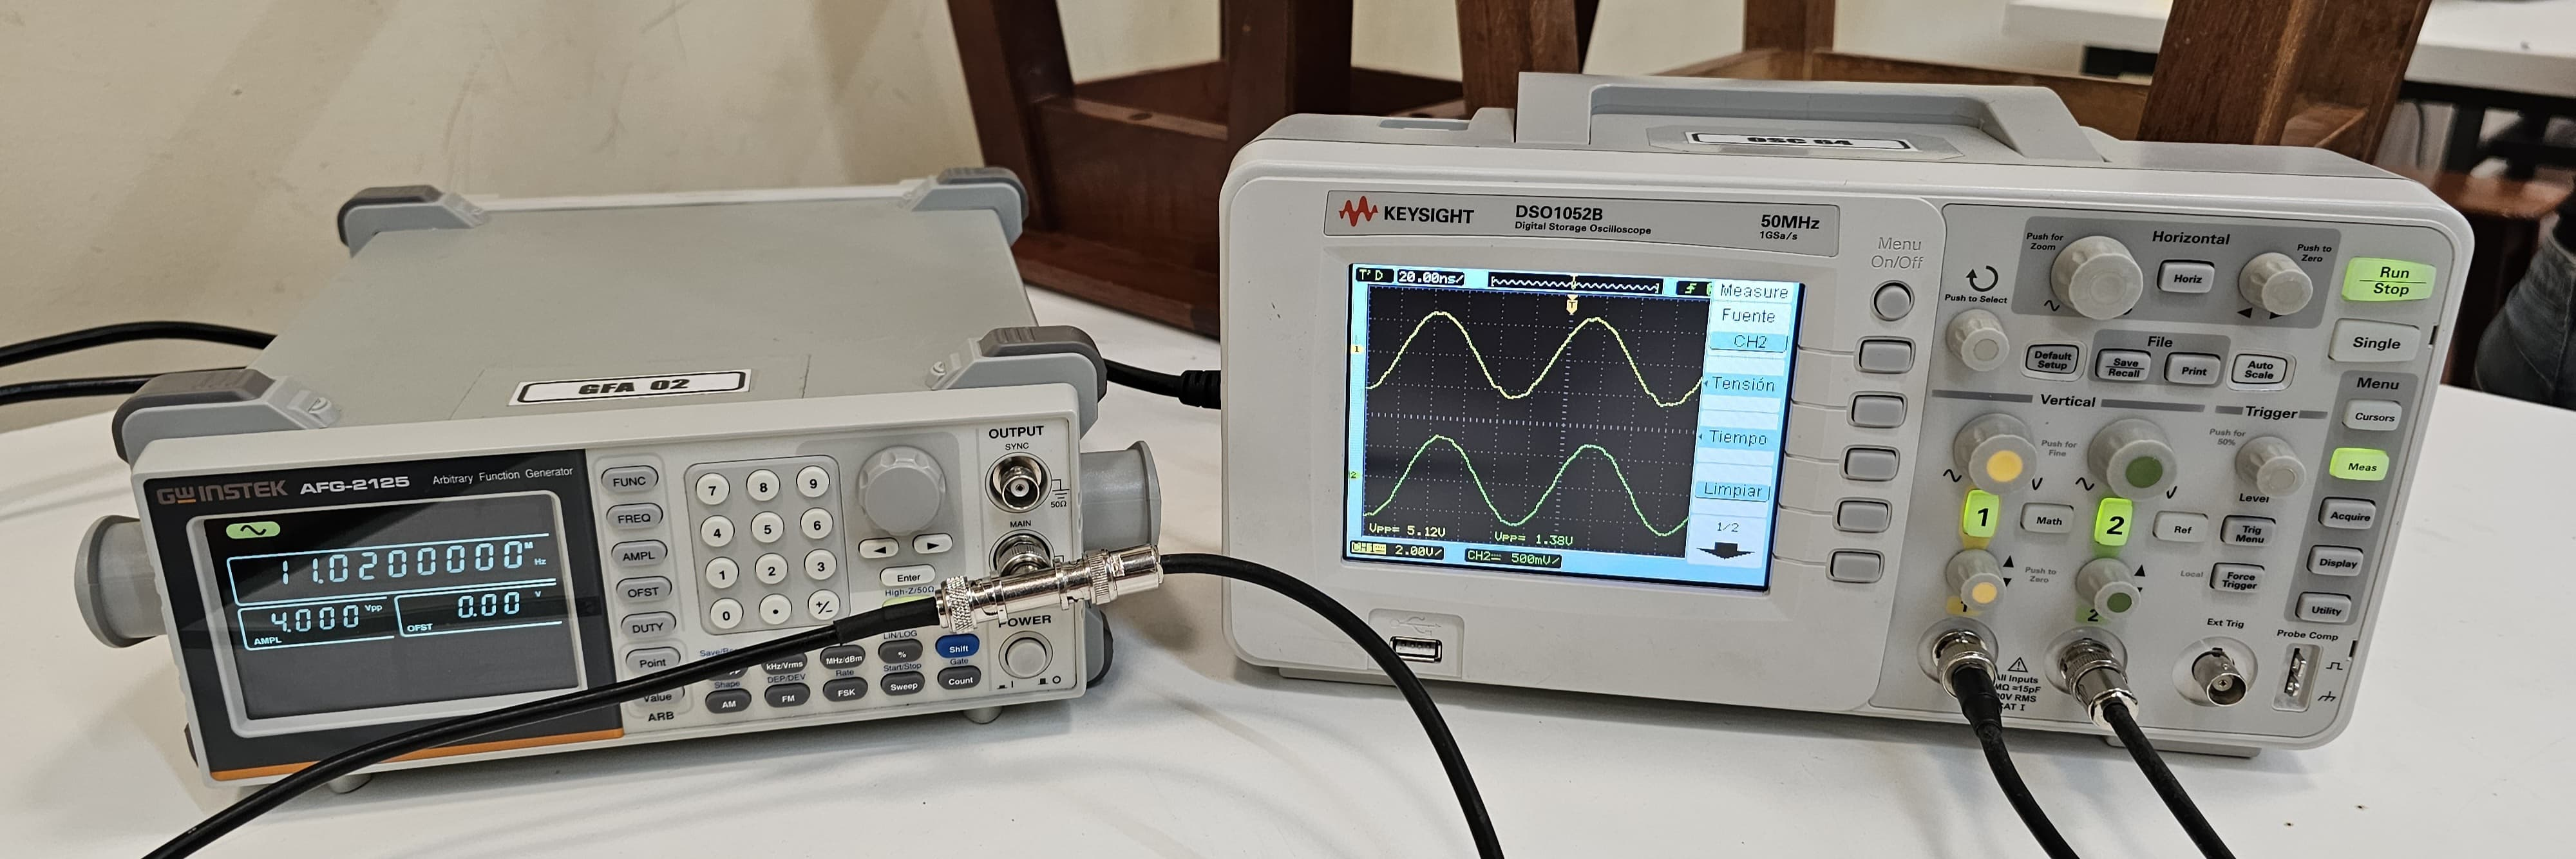
\includegraphics[width=0.9\textwidth]{./img/figura29.jpg}
\caption{Disposición de instrumentos durante las mediciones.}
\label{fig:circuito29}
\end{figure}
\subsection{Resultados}
\subsubsection{Resistencia de pérdidas}
Para la realización de este procedimiento, se utilizó un resistor de pruebas de $9.6 k\Omega$, obteniendo así lo siguiente:
\begin{itemize}
    \item $V_{out}=1.08 Vpp$
    \item $V_{in}=3.56 Vpp$
    \item $f_o=9.08 MHz$
\end{itemize}
\noindent Resulta en:
\begin{equation*}
    R_p = 4202.42 \Omega
\end{equation*}
\subsubsection{Inductancia, frecuencia de resonancia y factor de calidad descargado}
Se reutilizó el resistor de prueba de $9.6 k\Omega$, logrando así las siguientes mediciones:
\begin{itemize}
    \item $	f_{o1}=9.14 MHz$
    \item $	f_{o2}=6.34 MHz$
\end{itemize}
\noindent Con las frecuencias anteriores, se obtuvo:
\begin{equation*}
    C_x=164.54 pF
\end{equation*}
\begin{equation*}
    L=0.991 \mu F
\end{equation*}
\begin{equation*}
    f_o=13.44 MHz
\end{equation*}
\begin{equation*}
    Q_d=74.34
\end{equation*}
\noindent Es importante destacar que el capacitor físico utilizado es de $330 pF$.
\subsubsection{Impedancia de entrada}
Se encontró lo siguiente:
\begin{itemize}
    \item $	V_c=1.31 Vpp$
    \item $	V_d=3.52 Vpp$    
    \item $ f_o=11.02 MHz$
\end{itemize}
\noindent Obteniéndose así:
\begin{equation*}
    Z_{in}=29.64 \Omega
\end{equation*}
\subsubsection{Impedancia de salida}
Se midió:
\begin{itemize}
    \item $	V_c=4.2 Vpp$
    \item $	V_d=8.6 Vpp$
\end{itemize}
\noindent Entonces, a través de una medición directa se obtuvo el siguiente valor de la impedancia de salida:
\begin{equation*}
    Z_{out}=1047.62 \Omega
\end{equation*}
\subsubsection{Ancho de banda}
Se midió en frecuencia de resonancia ($11.02 MHz$), un valor de tensión de $V_{out}=4.2 Vpp$, lo que significa que, para encontrar las frecuencias de $3 dB$ de caída, se necesitó buscar una salida de $2.96 Vpp$. Se encontraron las siguientes frecuencias:
\begin{itemize}
    \item $f_1=10.69 MHz$
    \item $	f_2=11.72 MHz$
\end{itemize}
\noindent Que resultan en un ancho de banda de $1.03 MHz$, que implica un $Q_c=12.9$.
\subsubsection{Resumen de resultados}
Se muestra a continuación una tabla con los resultados de las mediciones obtenidas:
\begin{table}[h]
    \centering
    \label{tabla-1}
    \begin{tabular}{|l|l|}
    \hline
    $R_p$ & $4202.42 \Omega$ \\ \hline
    $C_x$ & $164.54 pF$ \\ \hline
    $L$ & $0.991 \mu Hy$ \\ \hline
    $f_o$ & $13.44 MHz$ \\ \hline
    $Q_d$ & $74.34$ \\ \hline
    $Z_{in}$ & $29.64 \Omega$ \\ \hline
    $Z_{out}$ & $1047.62 \Omega$ \\ \hline
    $BW$ & $1.03 MHz$ \\ \hline
    $Q_c$ & $12.9$ \\ \hline
    \end{tabular}
    \caption{Resumen de resultados obtenidos}
\end{table}
\newpage
Y, comparando con los valores planteados al inicio, en los requisitos de diseño, se tiene:
\begin{table}[h]
    \centering
    \label{tabla-2}
    \begin{tabular}{|l|l|l|l|}
    \hline
    \textbf{Magnitud} & \textbf{Valor de diseño} & \textbf{Valor obtenido} & \textbf{Variación} \\ \hline
    $R_p$ & $37324.55 \Omega$ & $4202.42 \Omega$ & -88.74\% \\ \hline
    $L$ & $0.978 \mu Hy$ & $0.991 \mu Hy$ & +1.33\% \\ \hline
    $f_o$ & $13 MHz$ & $13.44 MHz$ & +3.38\% \\ \hline
    $Z_{in}$ & $50 \Omega$ & $29.64 \Omega$ & -40.72\% \\ \hline
    $Z_{out}$ & $1000 \Omega$ & $1047.62 \Omega$ & +4.76\% \\ \hline
    $BW$ & $1.3 MHz$ & $1.03 MHz$ & -20.77\% \\ \hline
    $Q_c$ & $10$ & $12.9$ & +29\% \\ \hline
    $Q_d$ & $467.14$ & $74.34$ & -84.09\% \\ \hline
    \end{tabular}
    \caption{Comparación de valores de diseño y obtenidos}
\end{table}
\newpage
\section{Conclusiones}
Pudo completarse un trabajo práctico que consta de un circuito resonador a una determinada frecuencia. Sin embargo, los parámetros del sistema real difieren en cierta medida de lo obtenido mediante cálculos.

La parte considerada más complicada fue el bobinado del inductor, tarea que se torna dificil si no se cuenta con elementos apropiados para realizarla. Más allá de eso, no existieron otros inconvenientes. Se destaca la gran utilidad del carretel roscado impreso en 3D para poder mantener la separación uniforme entre espiras planteada en el diseño del inductor. Pudo comprobarse que el carretel hueco no afecta al valor de la inductancia, sin embargo, con los dispositivos de medición utilizado es muy dificil encontrar una variación de la frecuencia de resonancia, algo que evidentemente ocurre en la realidad, ya que la permeabilidad del plástico PLA no es la misma que la del aire. El agregado del carretel hueco hace que, en aproximadamente la misma frecuencia de resonancia, el valor de la tensión pico aumente con respecto a la situación en dónde éste no esté colocado. Esto se debe a que la resistencia de pérdidas del inductor aumenta con este agregado (probablemente porque la distancia entre espiras se mantiene constante, pudiendo tener un flujo magnético más uniforme), logrando que en el divisor resistivo (situación a la que se llega por la resonancia del circuito) aumente la caída de tensión en ese resistor.

La impedancia de entrada mostró una variación de 40\% con respecto a la original solicitada, esto puede deberse a dos factores principales:
\begin{itemize}
    \item Capacitancia parásita del osciloscopio: esta capacidad (como pudo medirse) tiene un valor comparable al resto de los capacitores utilizados, lo que termina afectando al circuito. Esta modificación que termina implicando el osciloscopio en el circuito real termina afectando las relaciones obtenidas como reflexiones de impedancia, no logrando la impedancia deseada en un principio.
    \item Resistencia de pérdidas distinta a la calculada: este valor difiere mucho del calculado para el diseño, lo que implica que la resistencia total del circuito termina variando, y por ese hecho se tiene un circuito muy diferente al simulado. 
\end{itemize}
\noindent Una manera de acercar el circuito un poco más al ideal calculado, eliminando la capacitancia parásita del osciloscopio es con un medidor de relación de onda estacionaria (ROE).

Las magnitudes de: impedancia de salida e inductancia (y, por ende, de frecuencia de resonancia) no se vieron muy afectadas con respecto a los parámetros de cálculo, esto puede deberse a la gran precisión con que está hecho el inductor, así como al valor casi redondo (con respecto al calculado) de los capacitores que reflejan la impedancia de salida.

El ancho de banda se vio modificado, esto por el hecho de que el factor de calidad descargado de la bobina no es exactamente el mismo que se pidió para el diseño. Como este factor depende directamente de la resistencia total e inversamente de la reactancia inductiva, puede entenderse que éste debería disminuir, ya que la resistencia total disminuye a causa de la gran reducción del valor de la resistencia de pérdidas del inductor. Este nuevo valor de $R_p$, que ahora resulta comparable a las demás resistencias que están en paralelo, hace que la resistencia resultante termine disminuyendo. Si disminuye la $R_T$, entonces también lo hace $Q_c$ en la misma medida, y, al darse esto, el ancho de banda debería aumentar, sin embargo, en la práctica ocurre el efecto totalmente contrario. Ocurre lo contrario porque las pérdidas no son extremadamente altas en la bobina, así que, para poder cumplir con el factor de calidad solicitado, y aumentar el ancho de banda, la solución más sencilla sería colocar un resistor en paralelo, de modo de disminuir aún más el valor de $Q_c$, y por ende aumentar el ancho de banda hasta llegar al valor solicitado.

En cuanto al factor de calidad descargado, puede verse una gran variación, que, a priori se puede predecir, ya que existió una gran diferencia entre el valor de la resistencia de pérdidas paralela del inductor real con respecto a la ideal. Esta variación de resistencia seguramente viene debida a cuestiones constructivas, así como de composición del material con el que se construyó el inductor, es algo sobre lo que no se tiene completo control.

Finalmente, de la tabla 2, puede hacerse un resumen de características e indicar si pasan o no una prueba de tolerancia, esto a modo de resumir el trabajo realizado. Se tiene entonces:

\begin{itemize}
    \item Resistencia de pérdidas: falla
    \item Inductancia: aprobada
    \item Frecuencia de resonancia: aprobada
    \item Impedancia de entrada: falla
    \item Impedancia de salida: aprobada marginal
    \item Ancho de banda: aprobado marginal
    \item Factor de calidad cargado: aprobado marginal
    \item Factor de calidad descargado: falla
    
\end{itemize}

\newpage

\begin{thebibliography}{9}
\bibitem{reference1}
Ing. Adolfo F. Gonzalez, Ing. Ricardo M. Cesari, Ing. Rubén O. Vicioli; \emph{Inductores con Núcleo de Aire, Revisión 2}, UTN Facultad Regional Mendoza, 2013.

\bibitem{reference2}
Ing. José Amado, Ing. Rodrigo Bruni; \emph{Apuntes de clase de la Cátedra de Electrónica Analógica III}, 2023.

\bibitem{reference3}
José B. Mariño; \emph{Adaptación de impedancias mediante redes selectivas}, E.T.S.I. de Telecomunicación de Tarrasa (Barcelona).

\bibitem{reference4}
Ing. Oscar M. Santa Cruz; \emph{Capítulo 11. Adaptación de impedancias}, 2010.

\end{thebibliography}

\end{document}